\documentclass[10pt,a4,uplatex]{jsarticle}
\usepackage{amsmath,amssymb}
%\usepackage{newtxtext,newtxmath}
\usepackage{bm} %太字のベクトル
%\usepackage{graphicx}
\usepackage[dvipdfmx]{graphicx}
\usepackage{ascmac} %枠囲み環境 itembox,screen,boxnote,shadebox
%\usepackage{fancyhdr}
%\pagestyle{fancy}
%\lhead{名前}
%\rhead{\today}
\usepackage{multicol}
\usepackage[top=15truemm,bottom=15truemm,left=15truemm,right=15truemm]{geometry}
%\setlength{\textwidth}{\fullwidth}
%\setlength{\textheight}{40\baselineskip}
%\addtolength{\textheight}{\topskip}
%\setlength{\voffset}{-0.2in}
%\setlength{\topmargin}{-0pt}
%\setlength{\headheight}{0pt}
%\setlength{\headsep}{0pt}
%
\usepackage{listings,jlisting}
\usepackage{color}

\lstset{
  breaklines = true,
  language={C++},
  basicstyle=\ttfamily\small,
  commentstyle={\itshape \color[cmyk]{1,0.4,1,0}},
  classoffset=1,
  keywordstyle={\bfseries \color[cmyk]{0,1,0,0}},
  stringstyle={\ttfamily \color[rgb]{0,0,1}},
  frame=tRBl,
  framesep=5pt,
  showstringspaces=false,
  numbers=left,
  stepnumber=1,
  numberstyle=\tiny,
  tabsize=2,
}

\title{生物情報科学演習 課題2 クラスタリング}
\author{生物情報科学科 05-145508 谷川洋介 (yk.tanigawa@gmail.com)}
\date{\today}
\begin{document}
\maketitle

\section{課題1 : 古典的なLloydの方法の実装}
\subsection{データ生成}
データの生成のために,次のようなプログラムを書いた。このプログラムは$n$個の点$\bm{x}_1, \bm{x}_2, \ldots, \bm{x}_n\quad(\forall{}i. \bm{x}_i\in[0,1]^d)$をC++11の乱数ライブラリのメルセヌスツイスタを用いて生成する。生成されたデータは,ファイルに書きだされる。

データの個数$n$,次元の大きさ$d$は引数として与える。また,reproducible researchの観点から重要である,乱数のシードも引数として与えることができる。プログラムがデータの生成の際に使用したシードの値は標準出力に表示される。
\lstinputlisting[caption=rand\_data\_generator.cpp (データ生成のためのプログラム)]
{../program/rand_data_generator.cpp}

\subsection{プログラムの実装}
ベクトルの和などの基本的な演算は,ヘッダーファイル\verb+my_vector.hpp+内に実装した。
\lstinputlisting[caption=my\_vector.hpp (ベクトルの基本演算)]
{../program/my_vector.hpp}

プログラムの実行時間を計測するためのサブルーチンは,ヘッダーファイル\verb+time_bench.hpp+内に実装した。
\lstinputlisting[caption=time\_bench.hpp (実行時間計測のためのサブルーチン)]
{../program/time_bench.hpp}

プログラムの本体は,\verb+Lloyd.cpp+内に実装した。
\lstinputlisting[caption=Lloyd.cpp (LloydのK-meansアルゴリズム)]
{../program/Lloyd.cpp}


\subsection{プログラムの実行}
下記のようなシェルスクリプトによりプログラムを実行した。レポートとして提出するファイルの中には,生成したデータファイルは含まれていない。
\lstinputlisting[language={bash}, caption=exec.sh (プログラムの実行のためのスクリプト)]
{../program/exec.sh}

\subsection{実行結果}
プログラムの実行結果を次に示す。各列は順に,$n$(データサイズ),$d$(次元), $k$(クラスタ数), プログラム実行時間(マイクロ秒単位), 平均二乗誤差, 収束に要した繰り返し回数を表している。ただし,$n = 100000, d = 100, k = 1000$のケースについては,プログラムの実行時間がとても長くなったので途中で実行を中止したため,データがない。

\lstinputlisting[caption=results.txt (プログラムの実行結果)]
{../results.txt}

\subsection{データの解析}
\subsubsection{Rによるデータのプロット}
先の節で得た結果を解釈するために,Rを用いてグラフを作成した。下記のプロットに用いたスクリプトを示す。
\lstinputlisting[language={R}, caption=analysis.R (プロット用のスクリプト)]
{../analysis.R}

\subsubsection{プロットした結果}
\begin{figure}[!htbp]
  \centering %
  \begin{tabular}{ccc}
      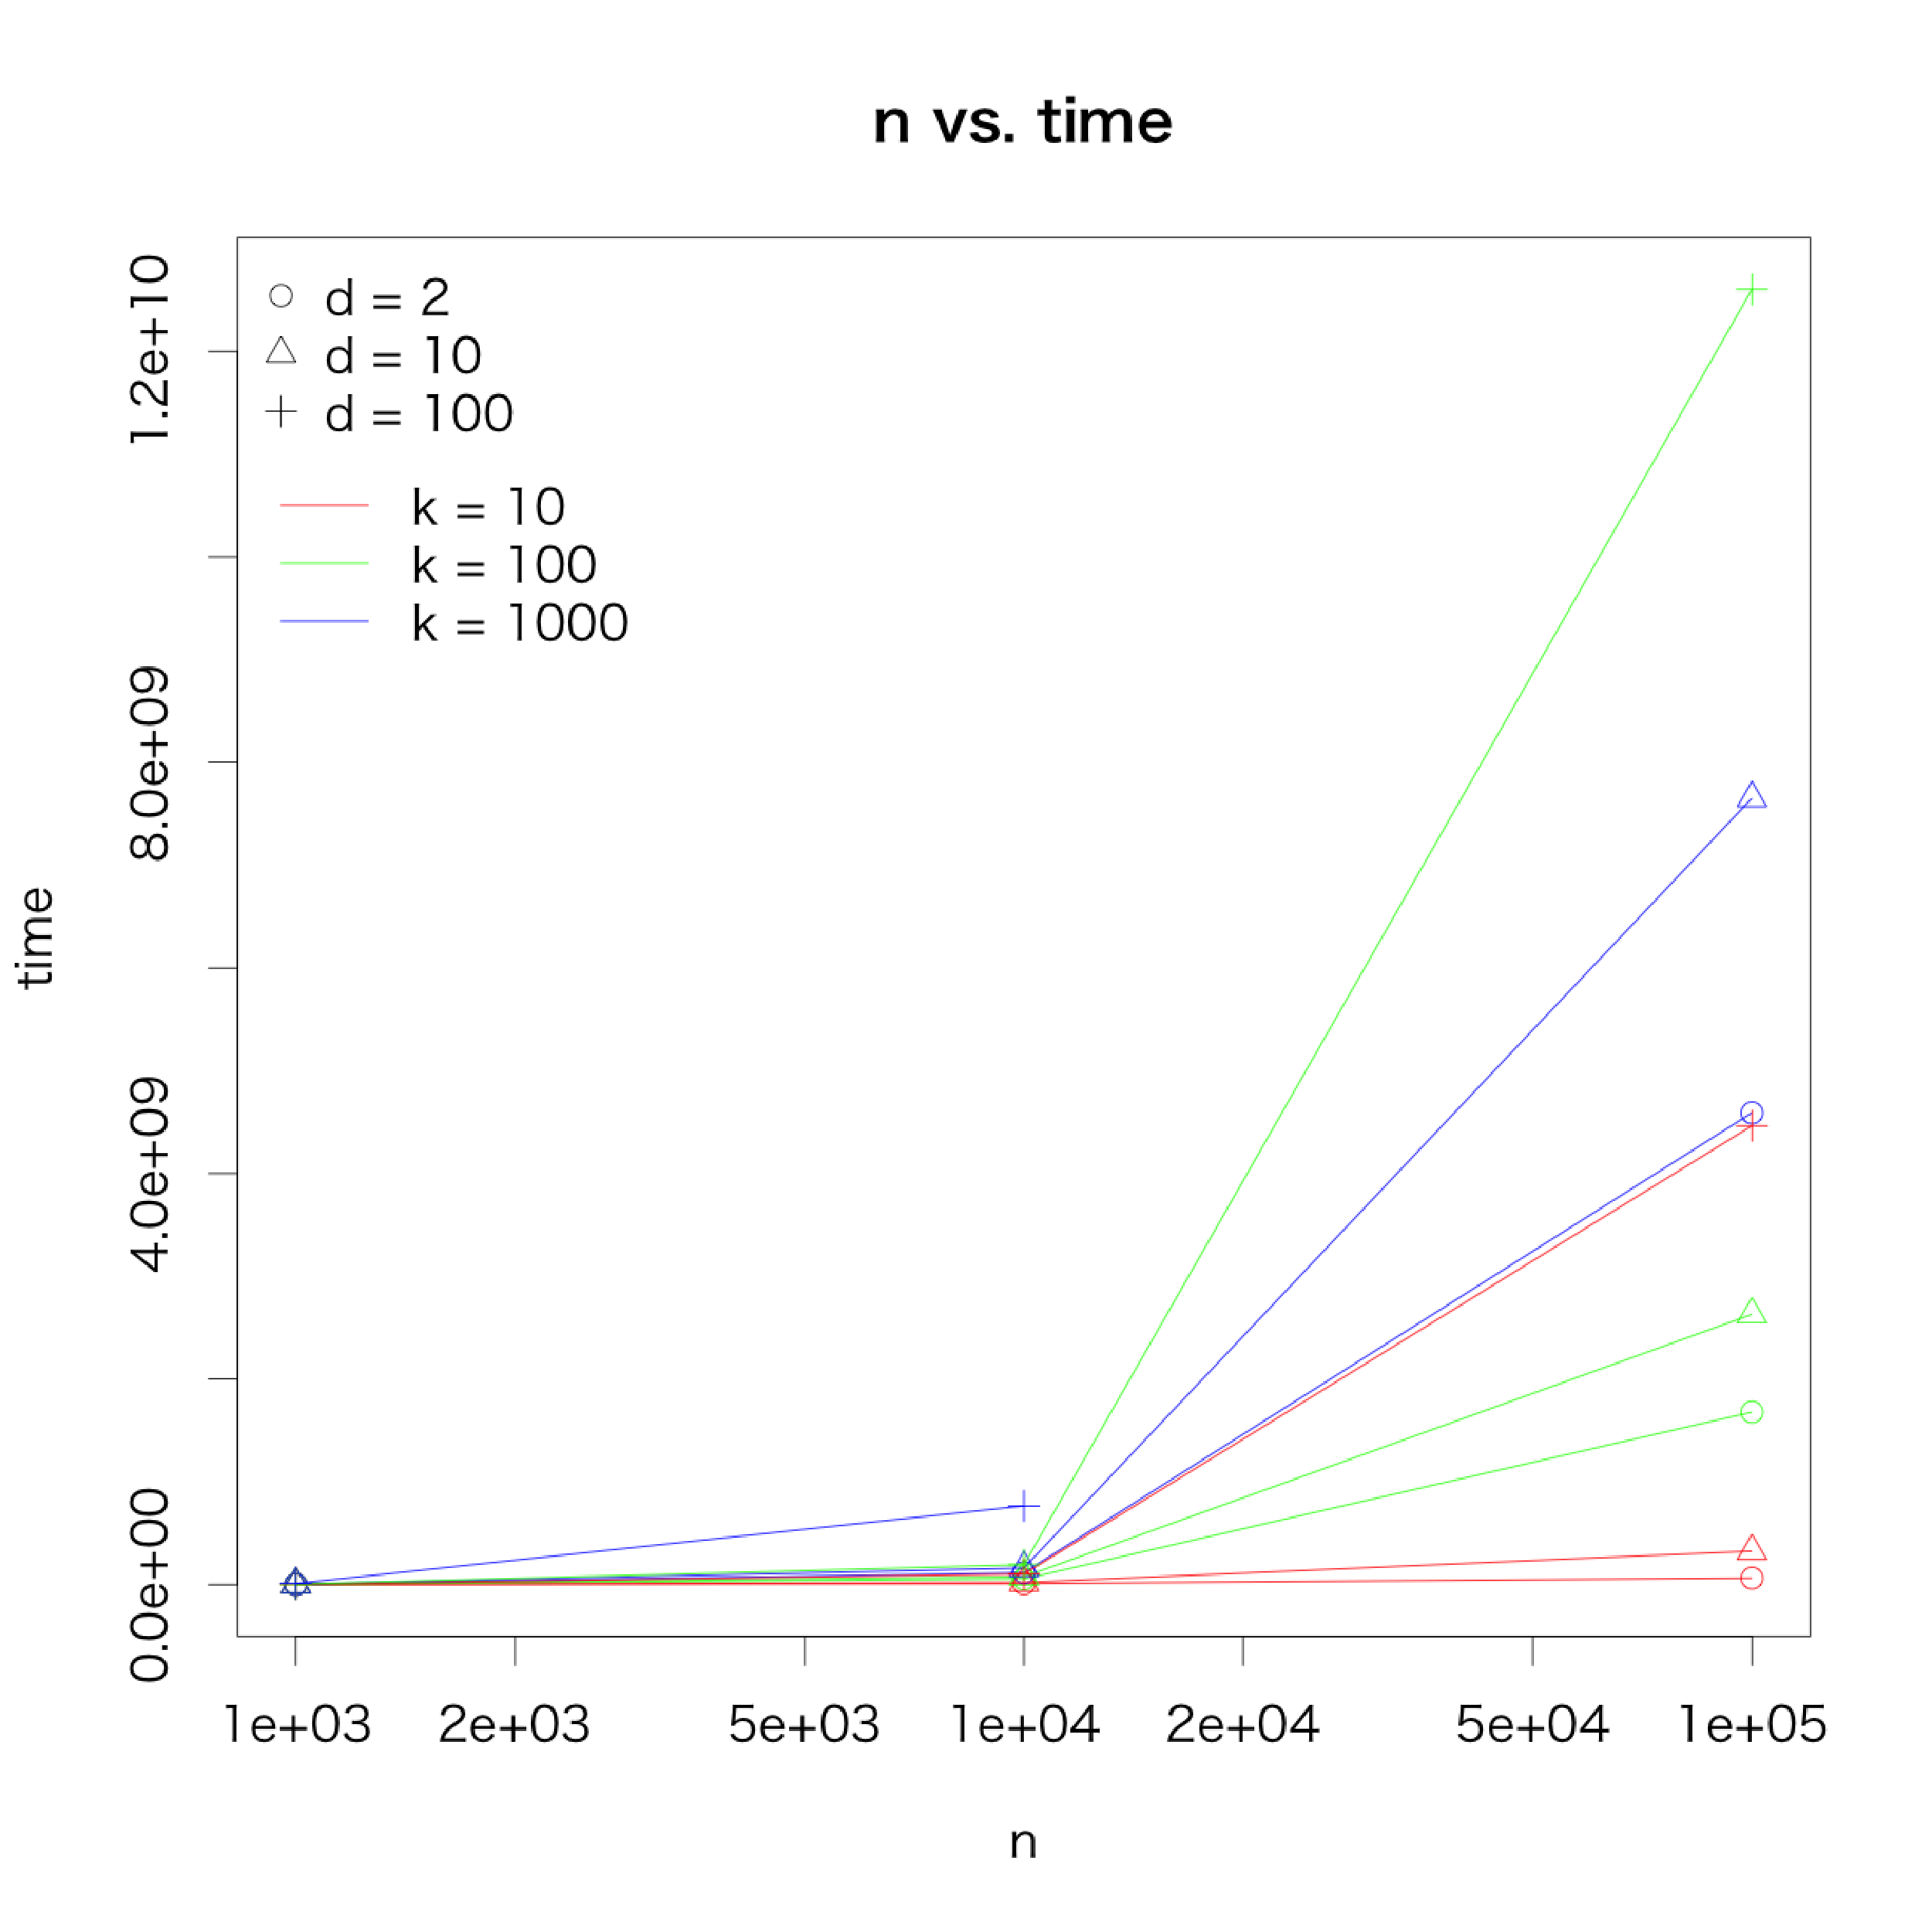
\includegraphics[width=0.33\hsize]{./n_time.pdf}
      &
      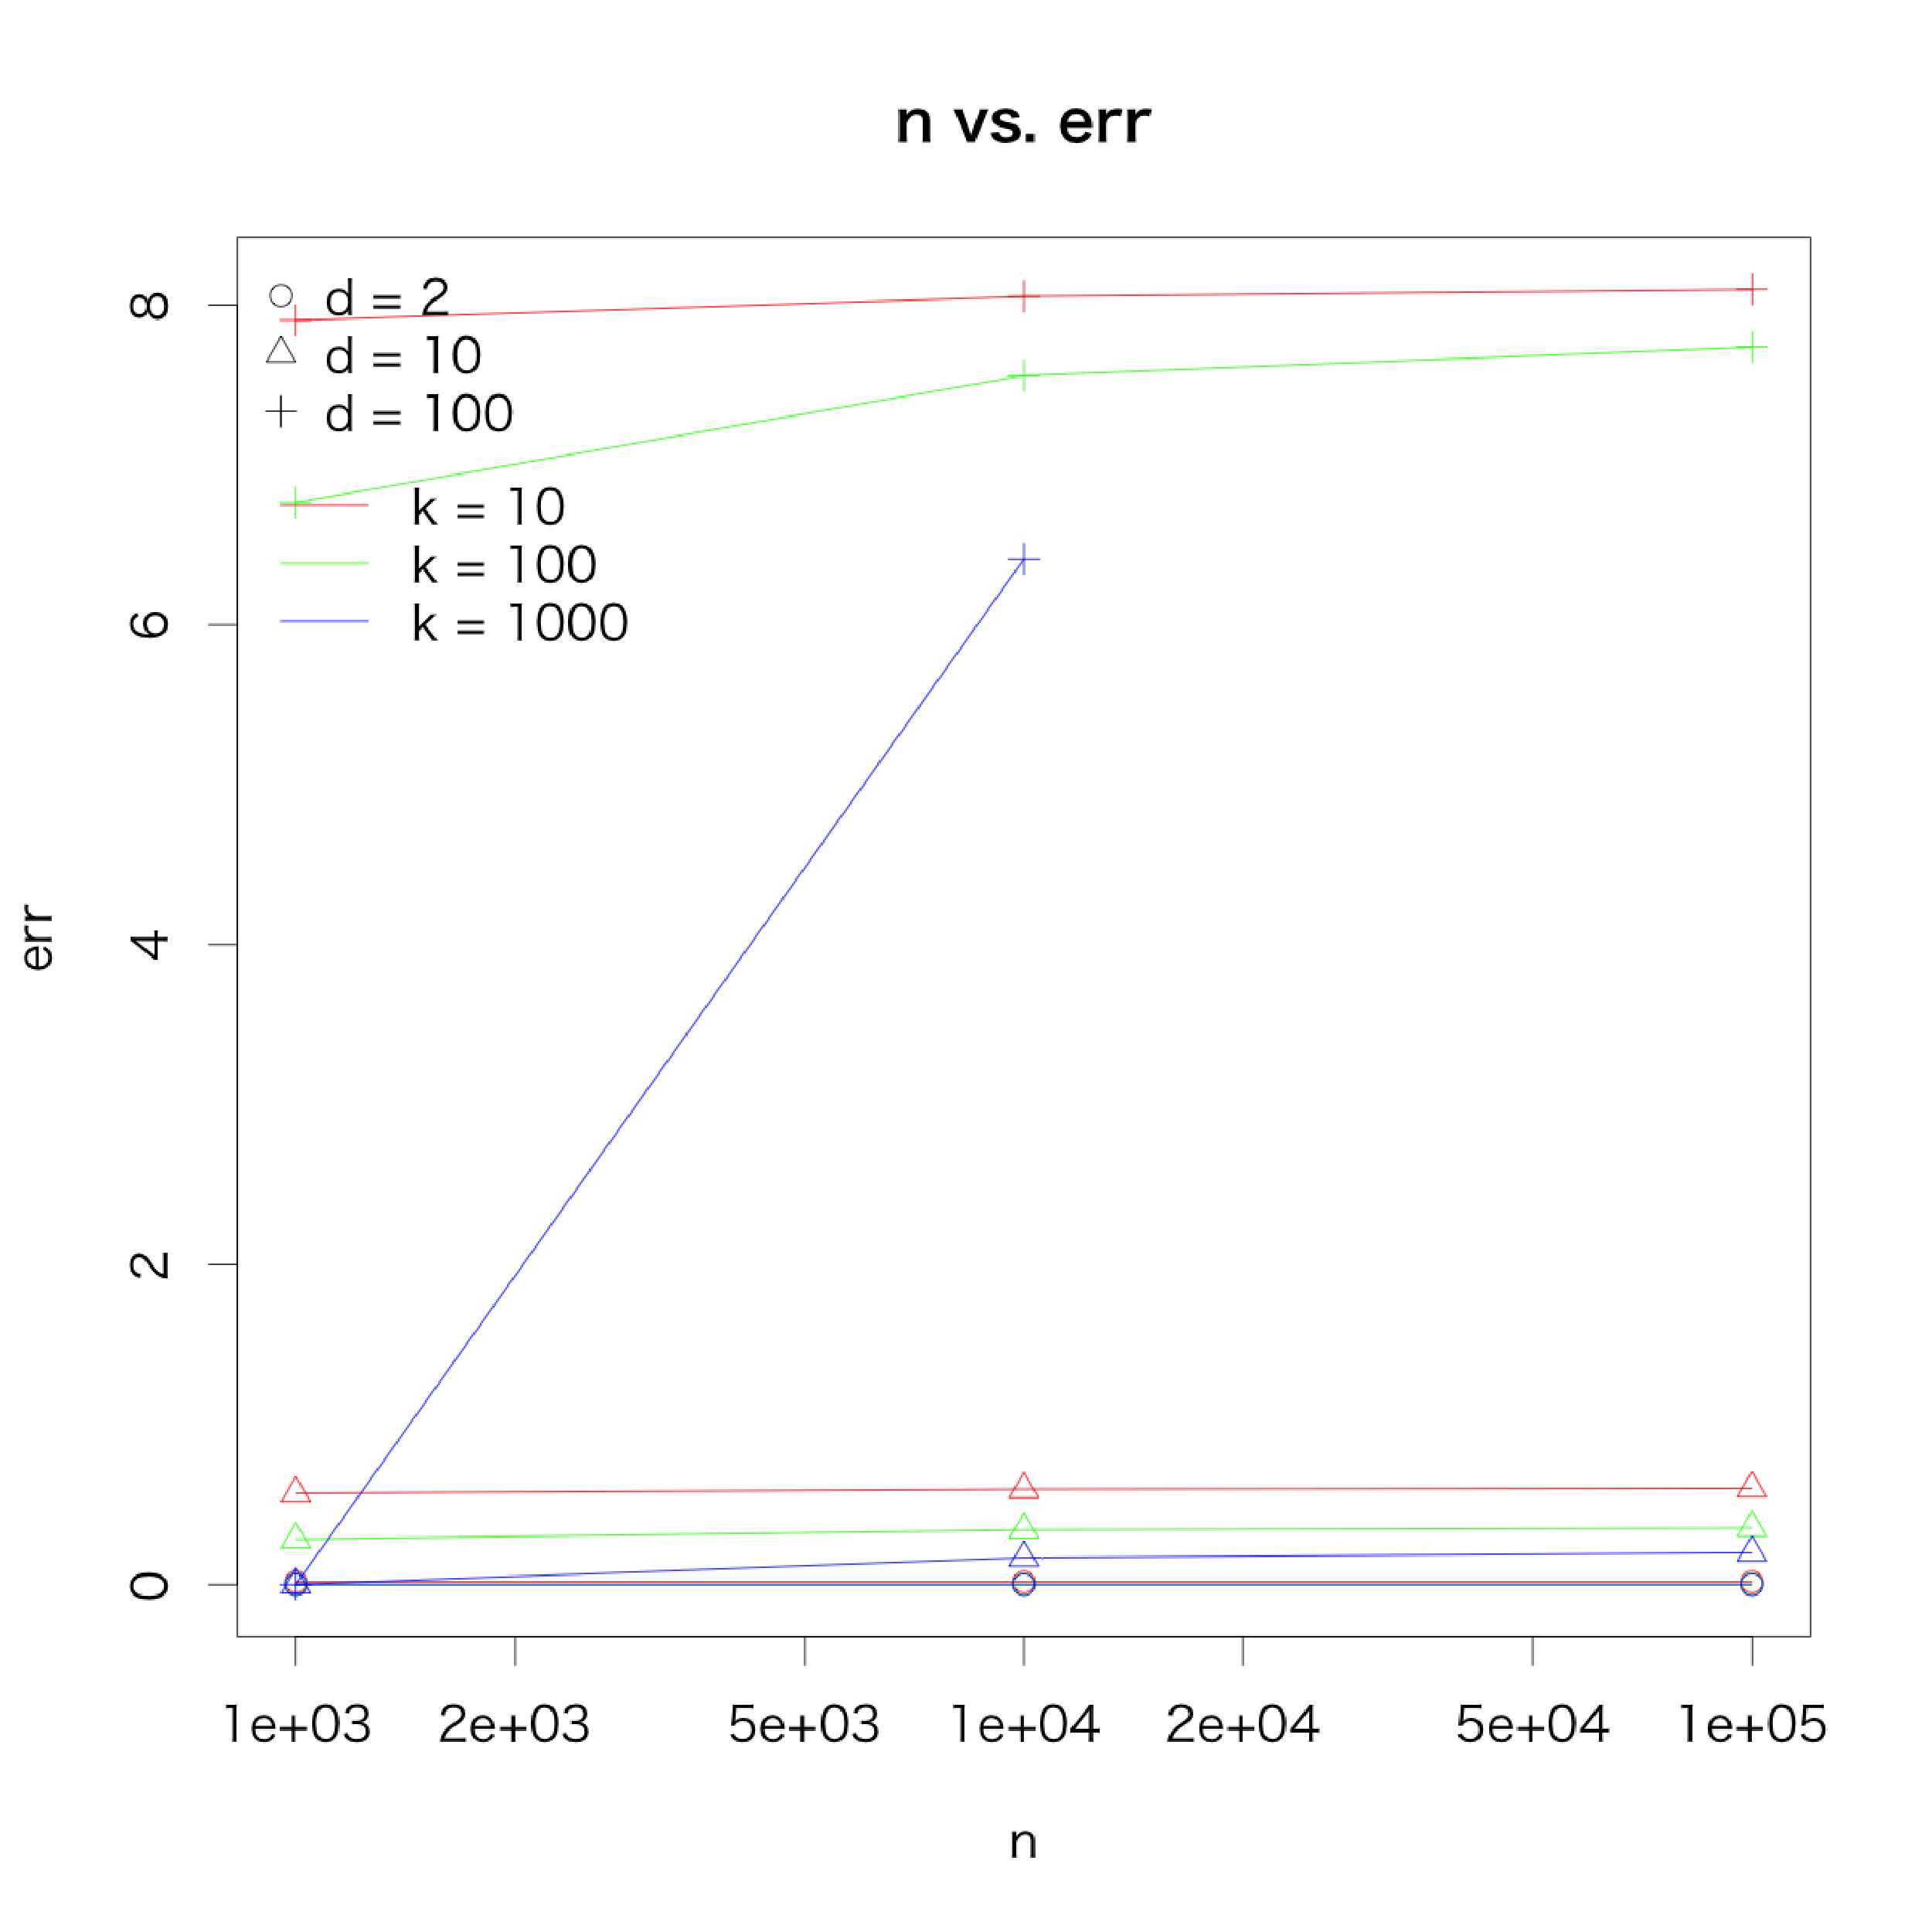
\includegraphics[width=0.33\hsize]{./n_err.pdf}
      &
      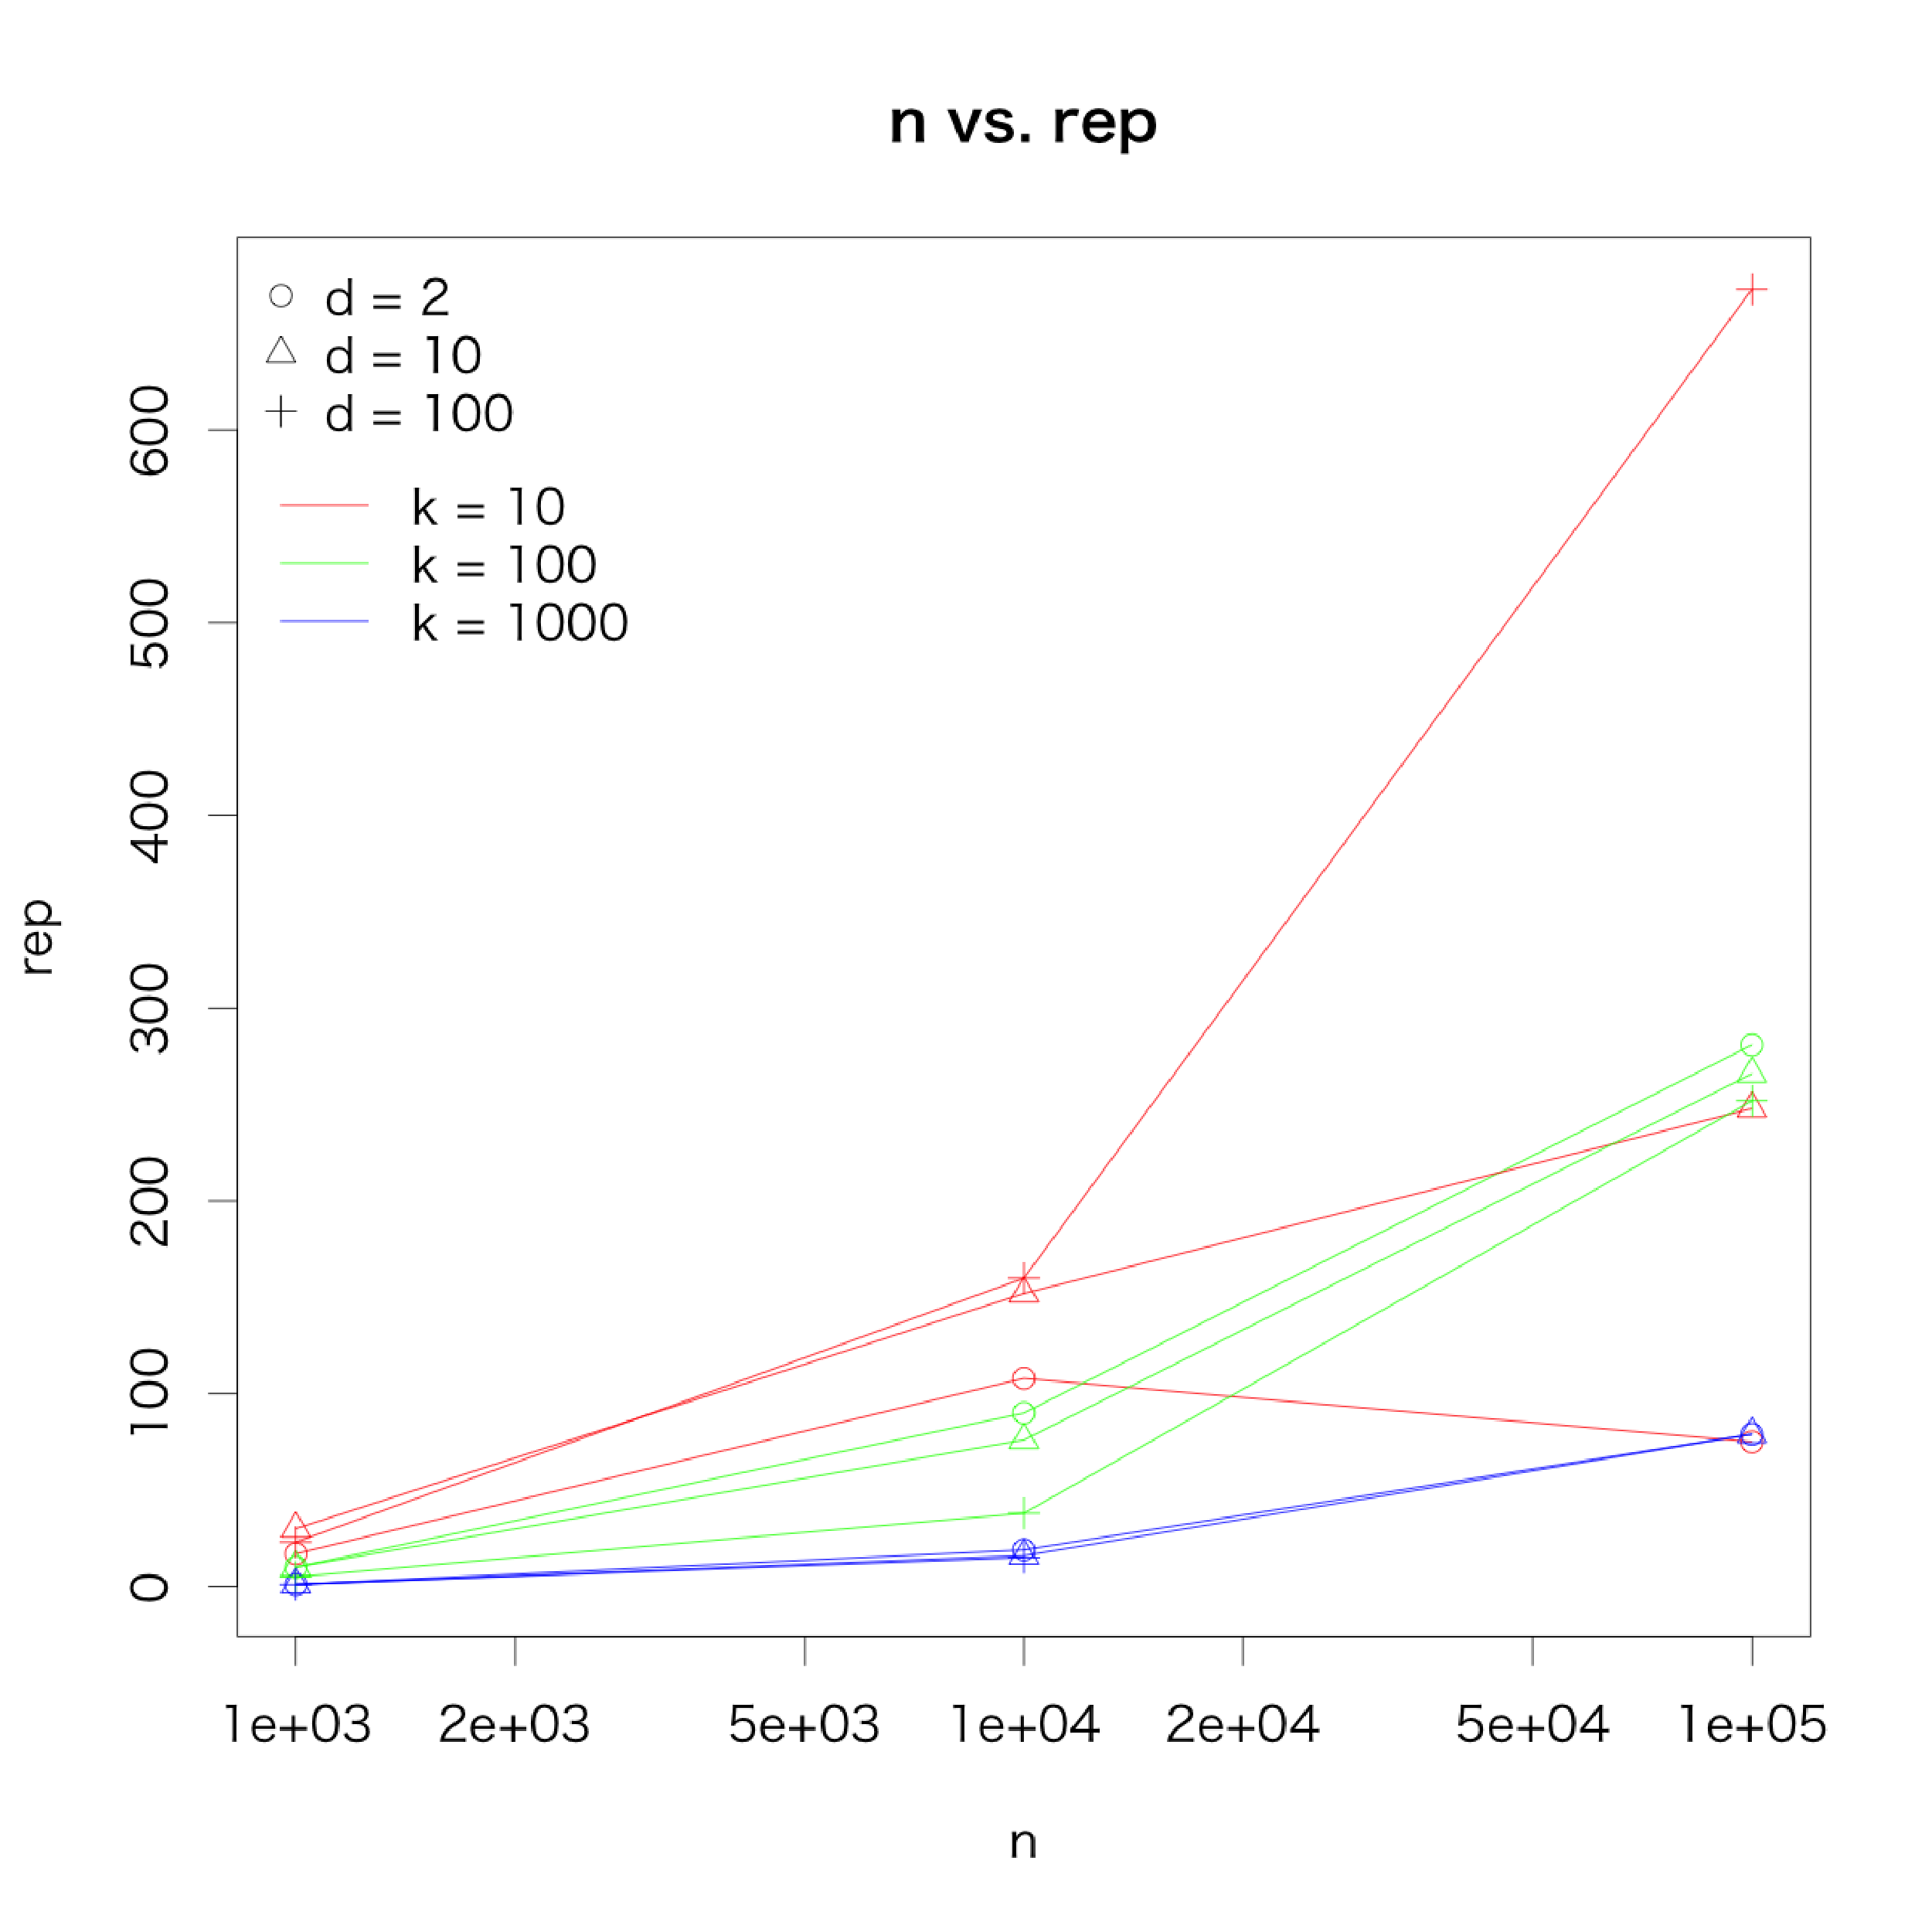
\includegraphics[width=0.33\hsize]{./n_rep.pdf}
    \\
      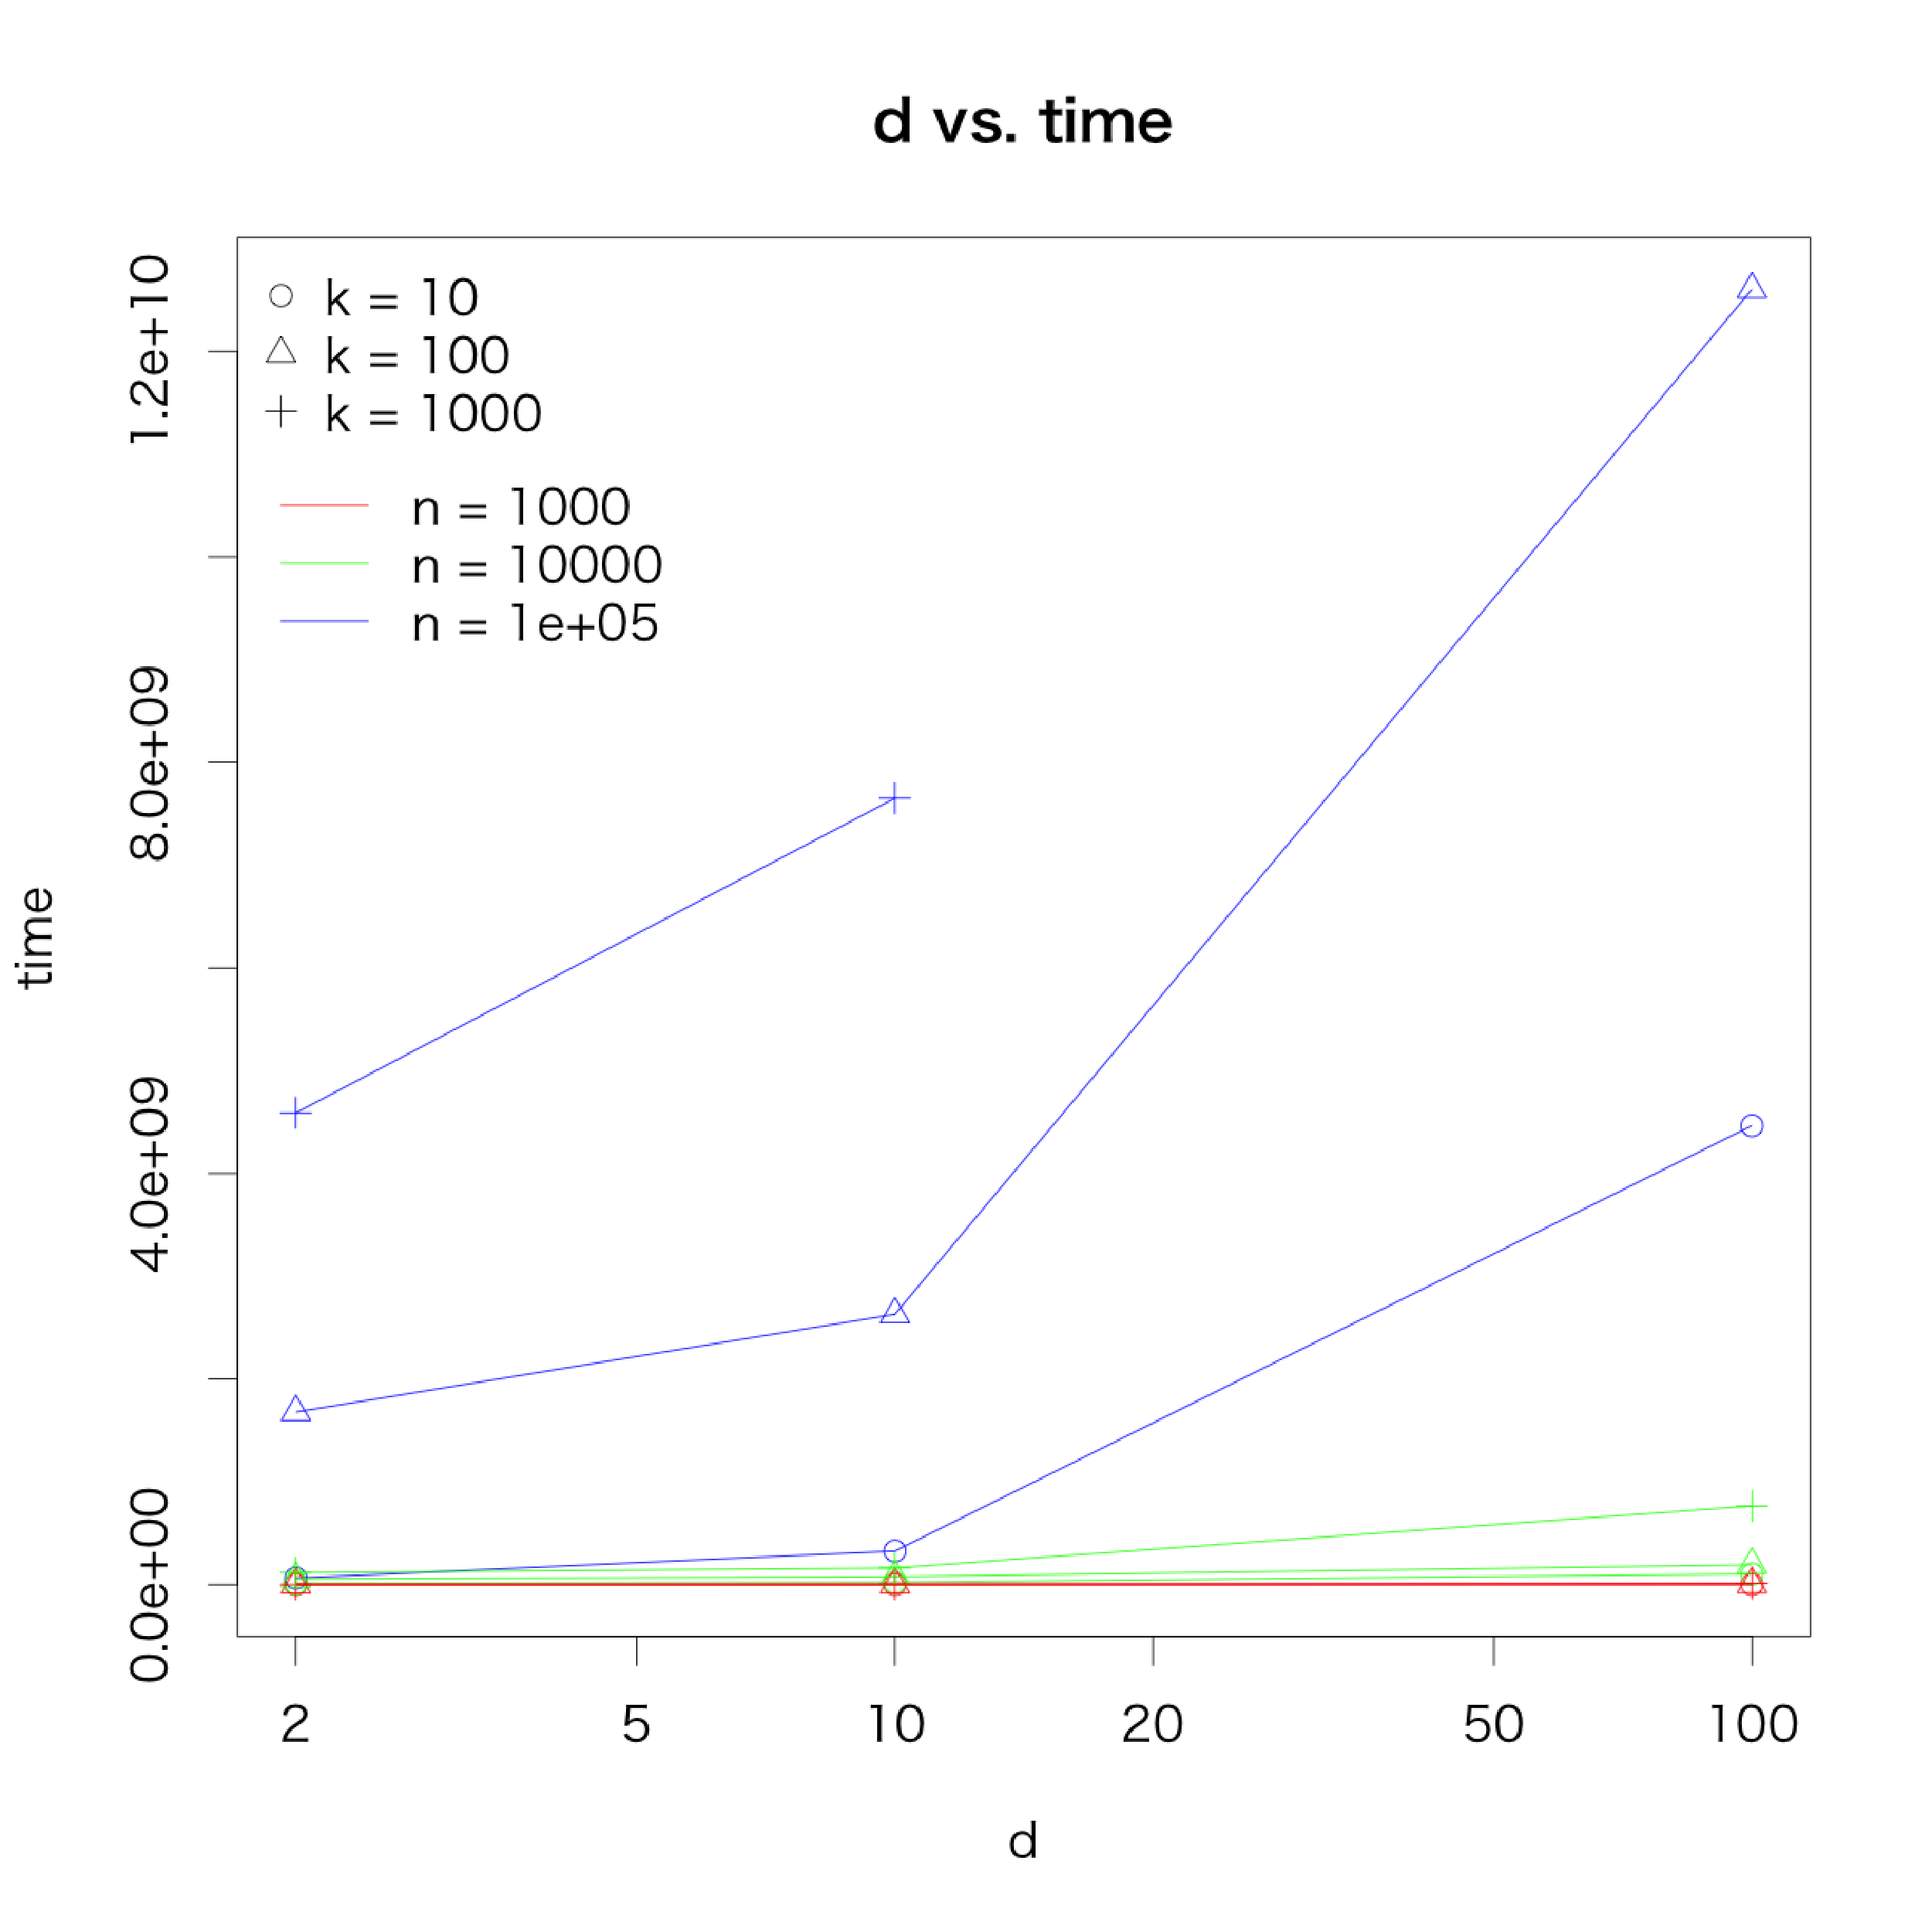
\includegraphics[width=0.33\hsize]{./d_time.pdf}
      &
      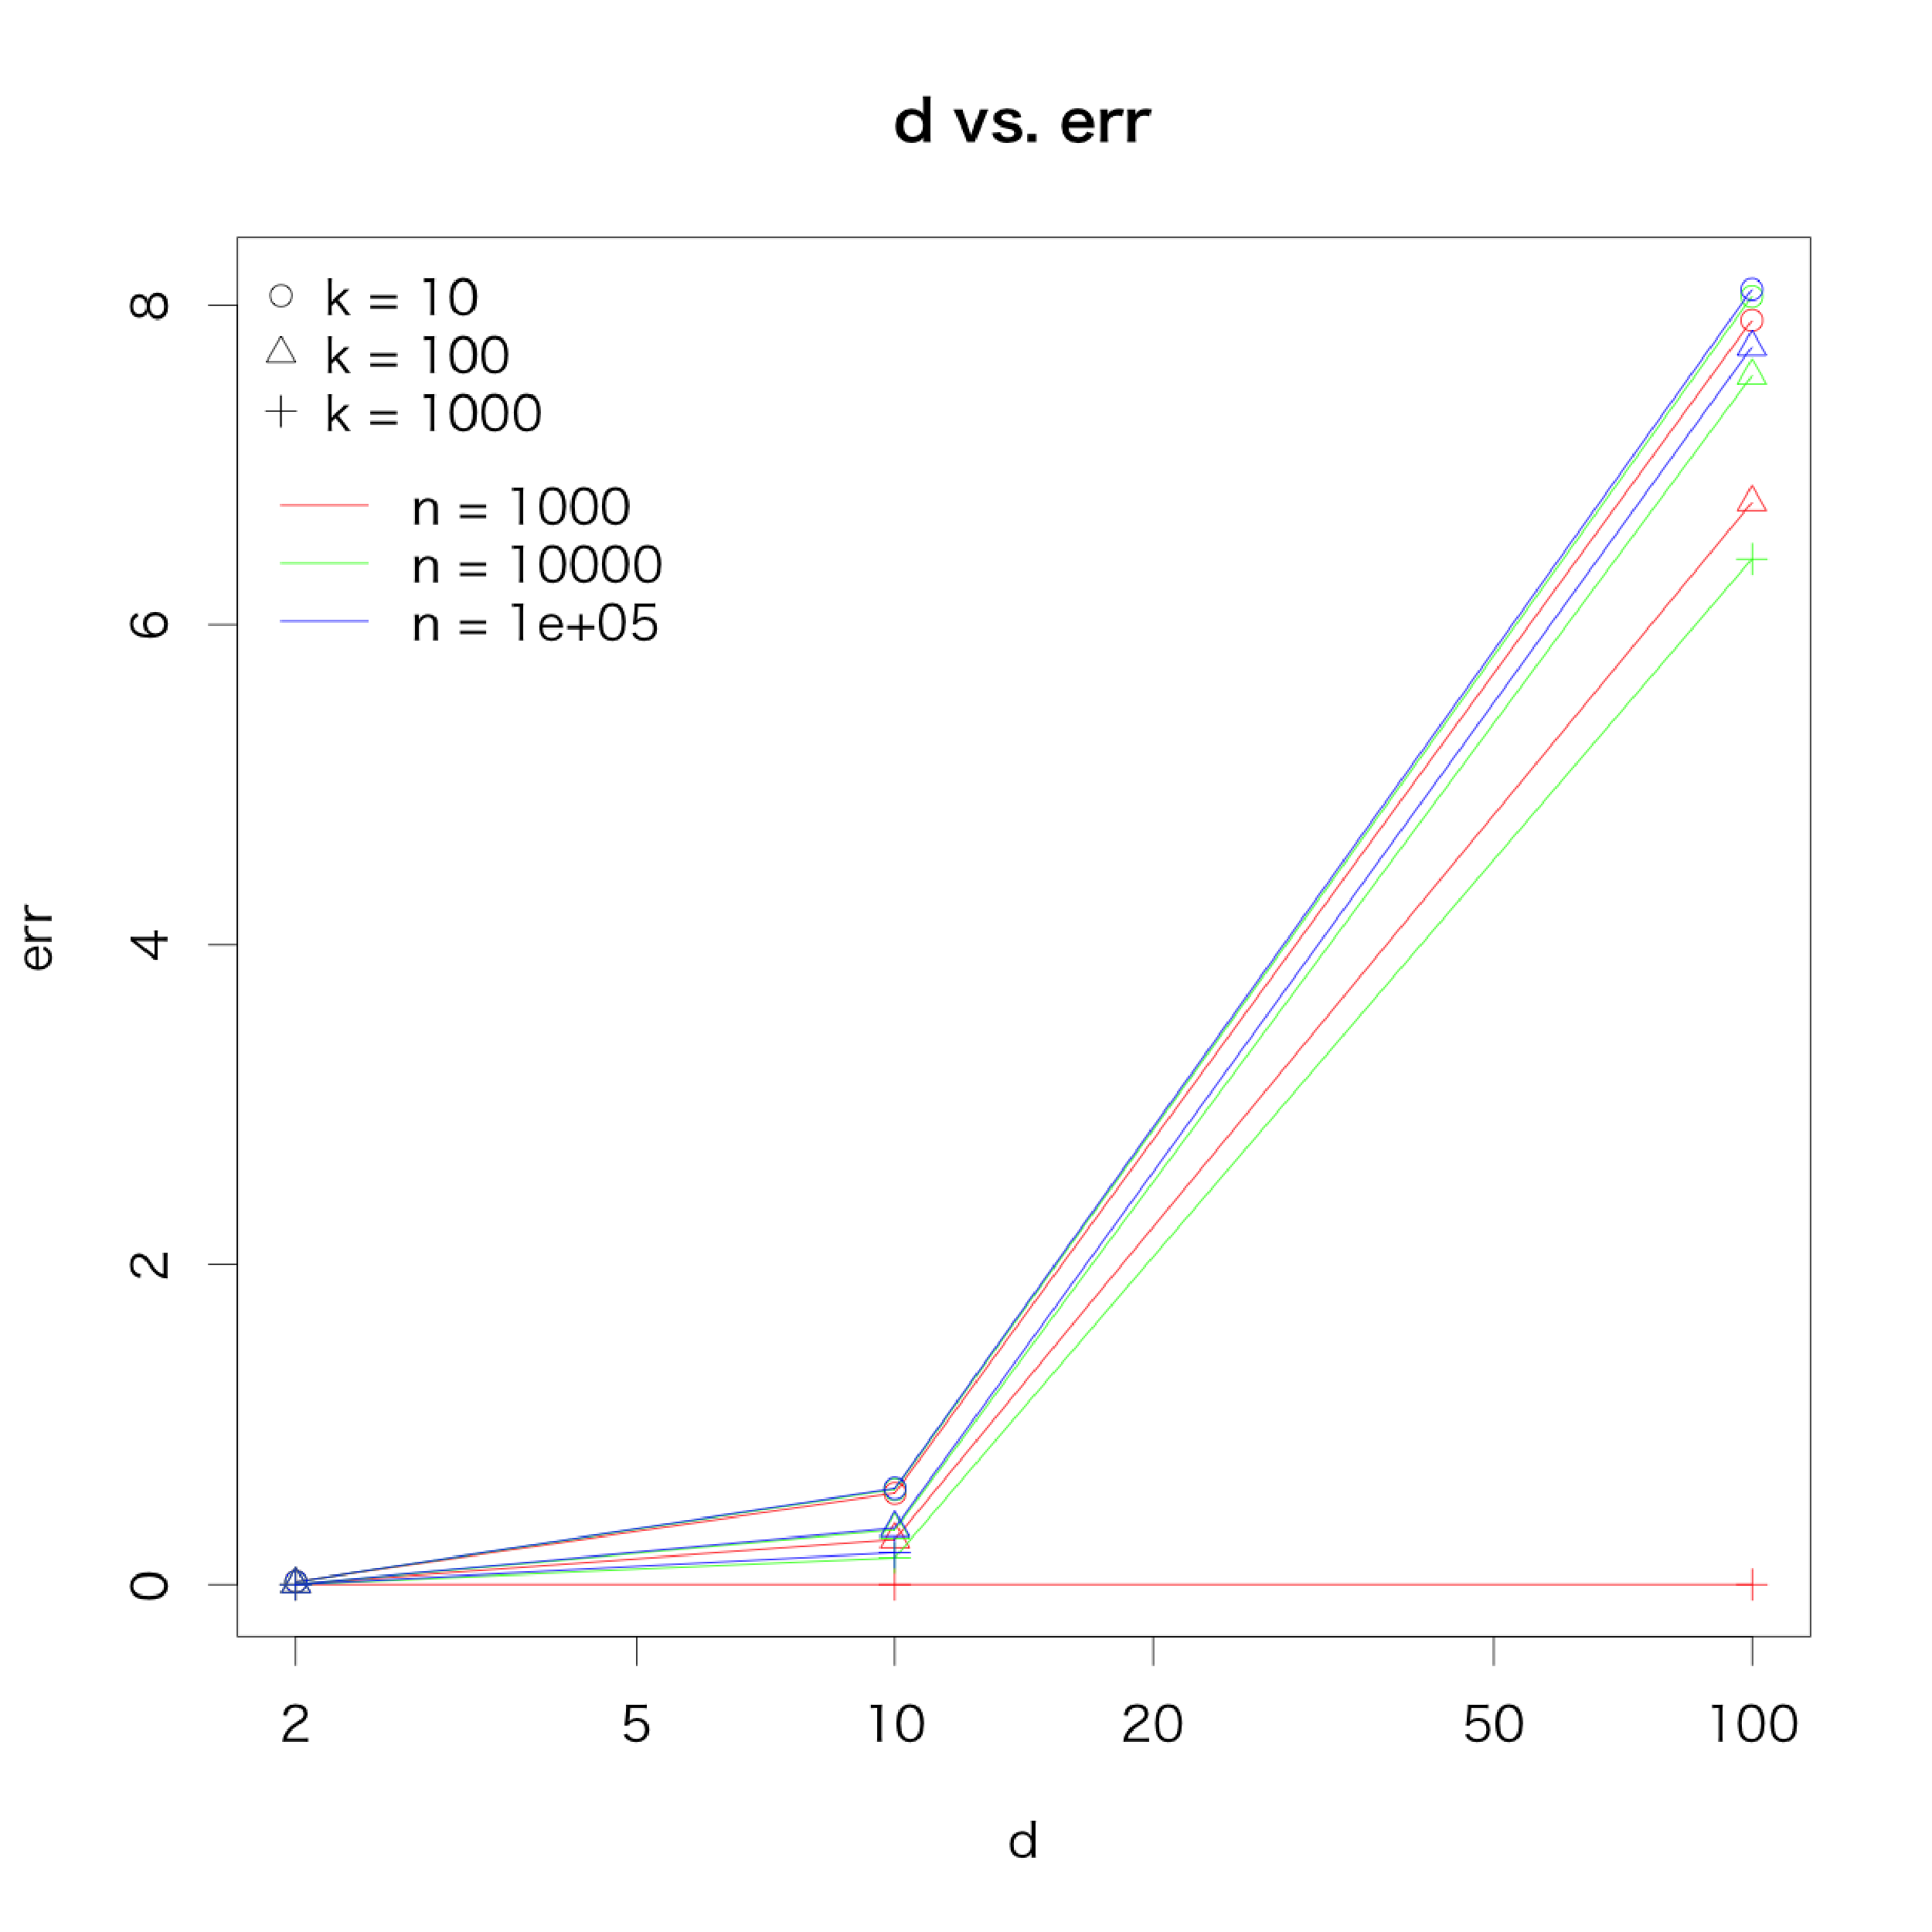
\includegraphics[width=0.33\hsize]{./d_err.pdf}
      &
      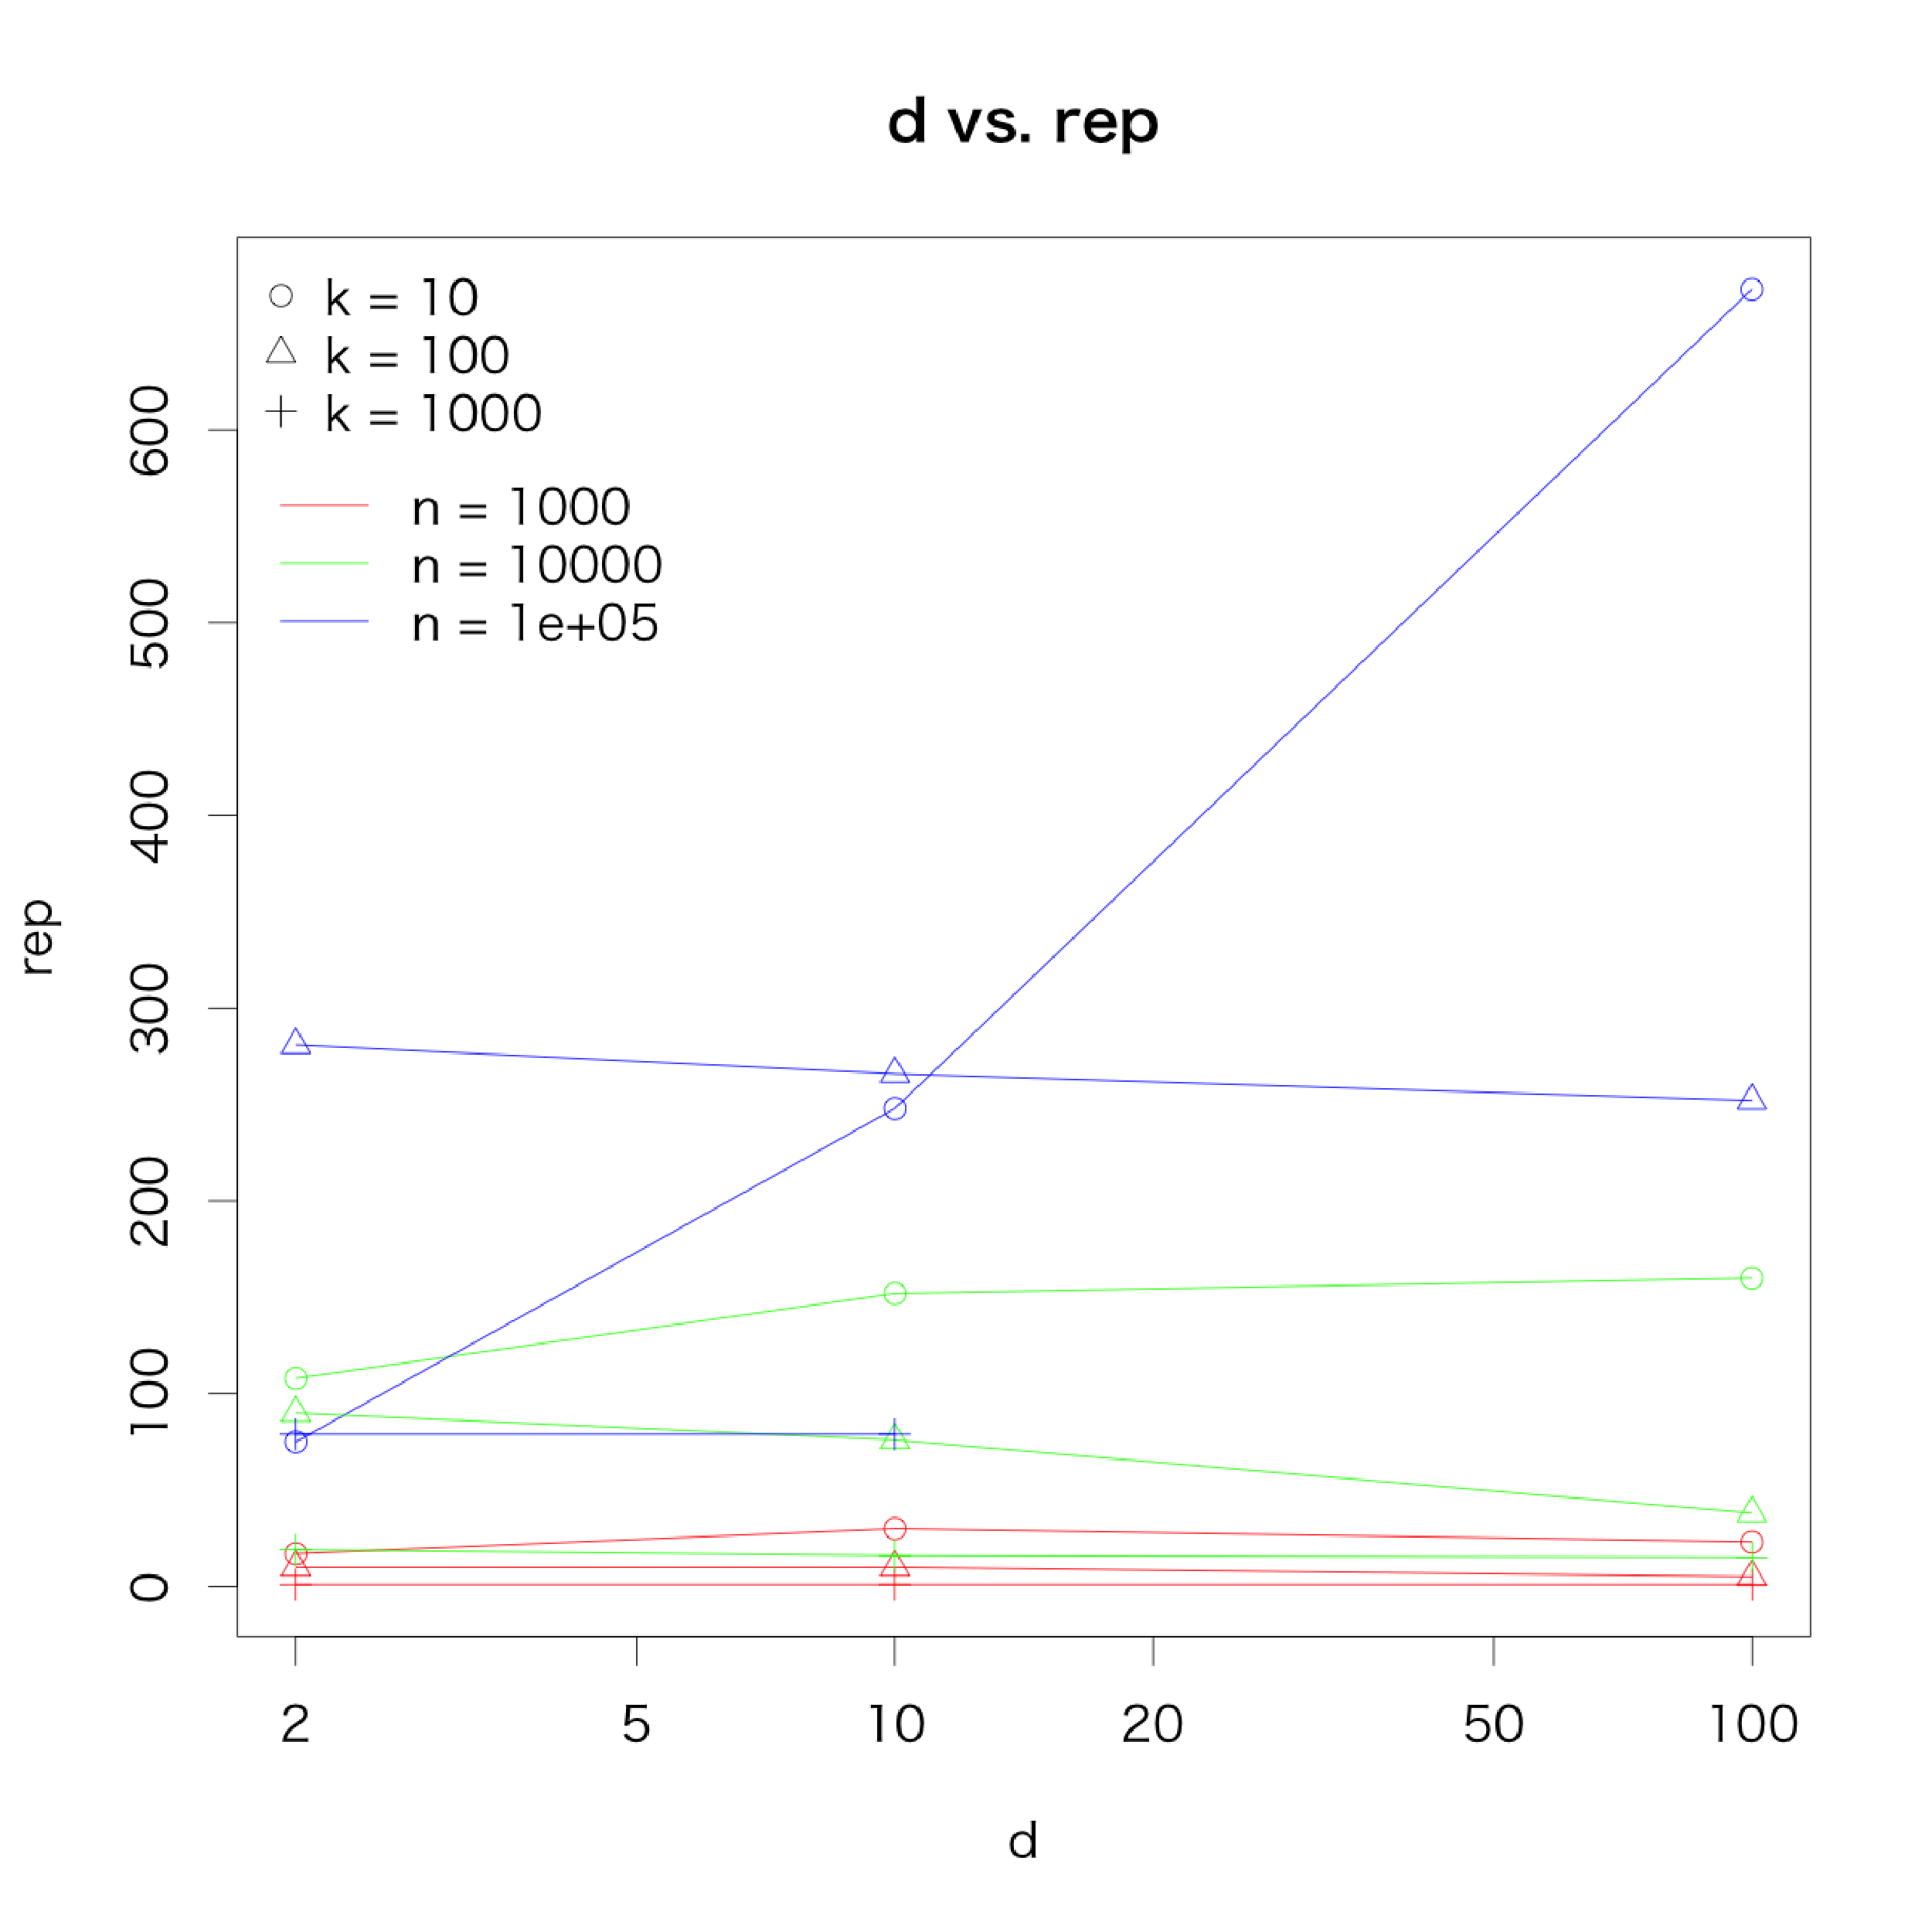
\includegraphics[width=0.33\hsize]{./d_rep.pdf}
    \\
      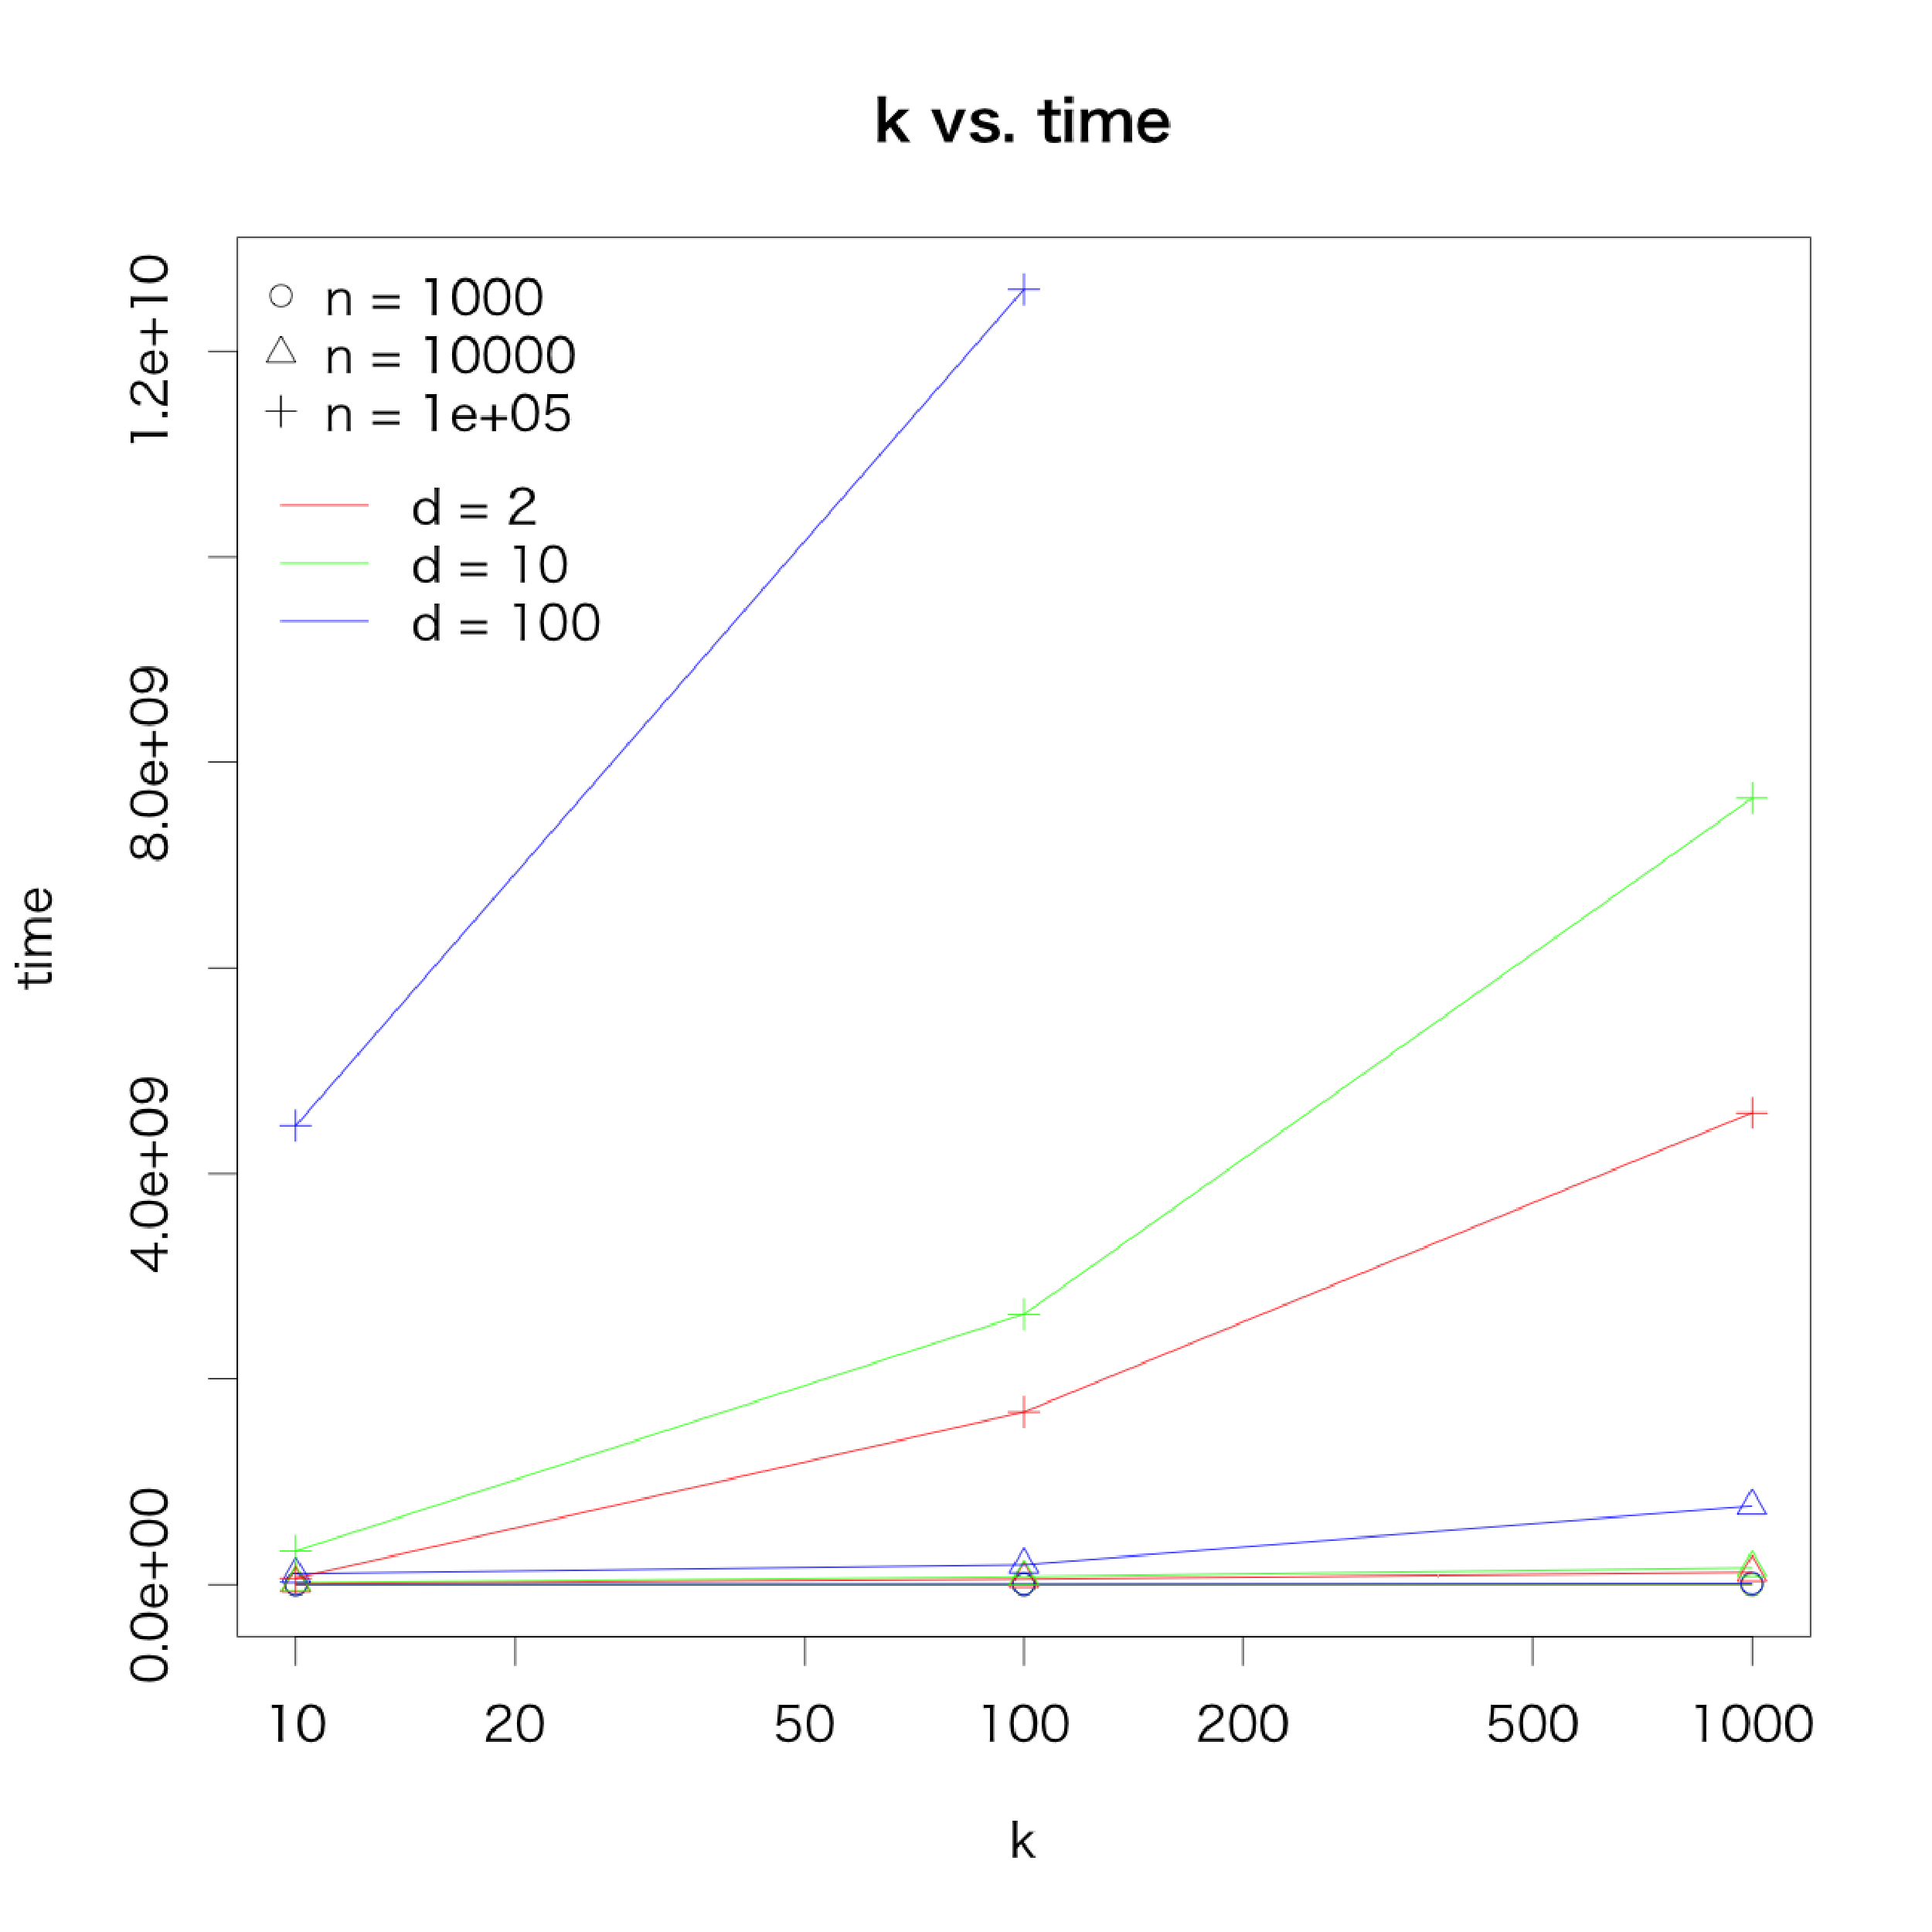
\includegraphics[width=0.33\hsize]{./k_time.pdf}
      &
      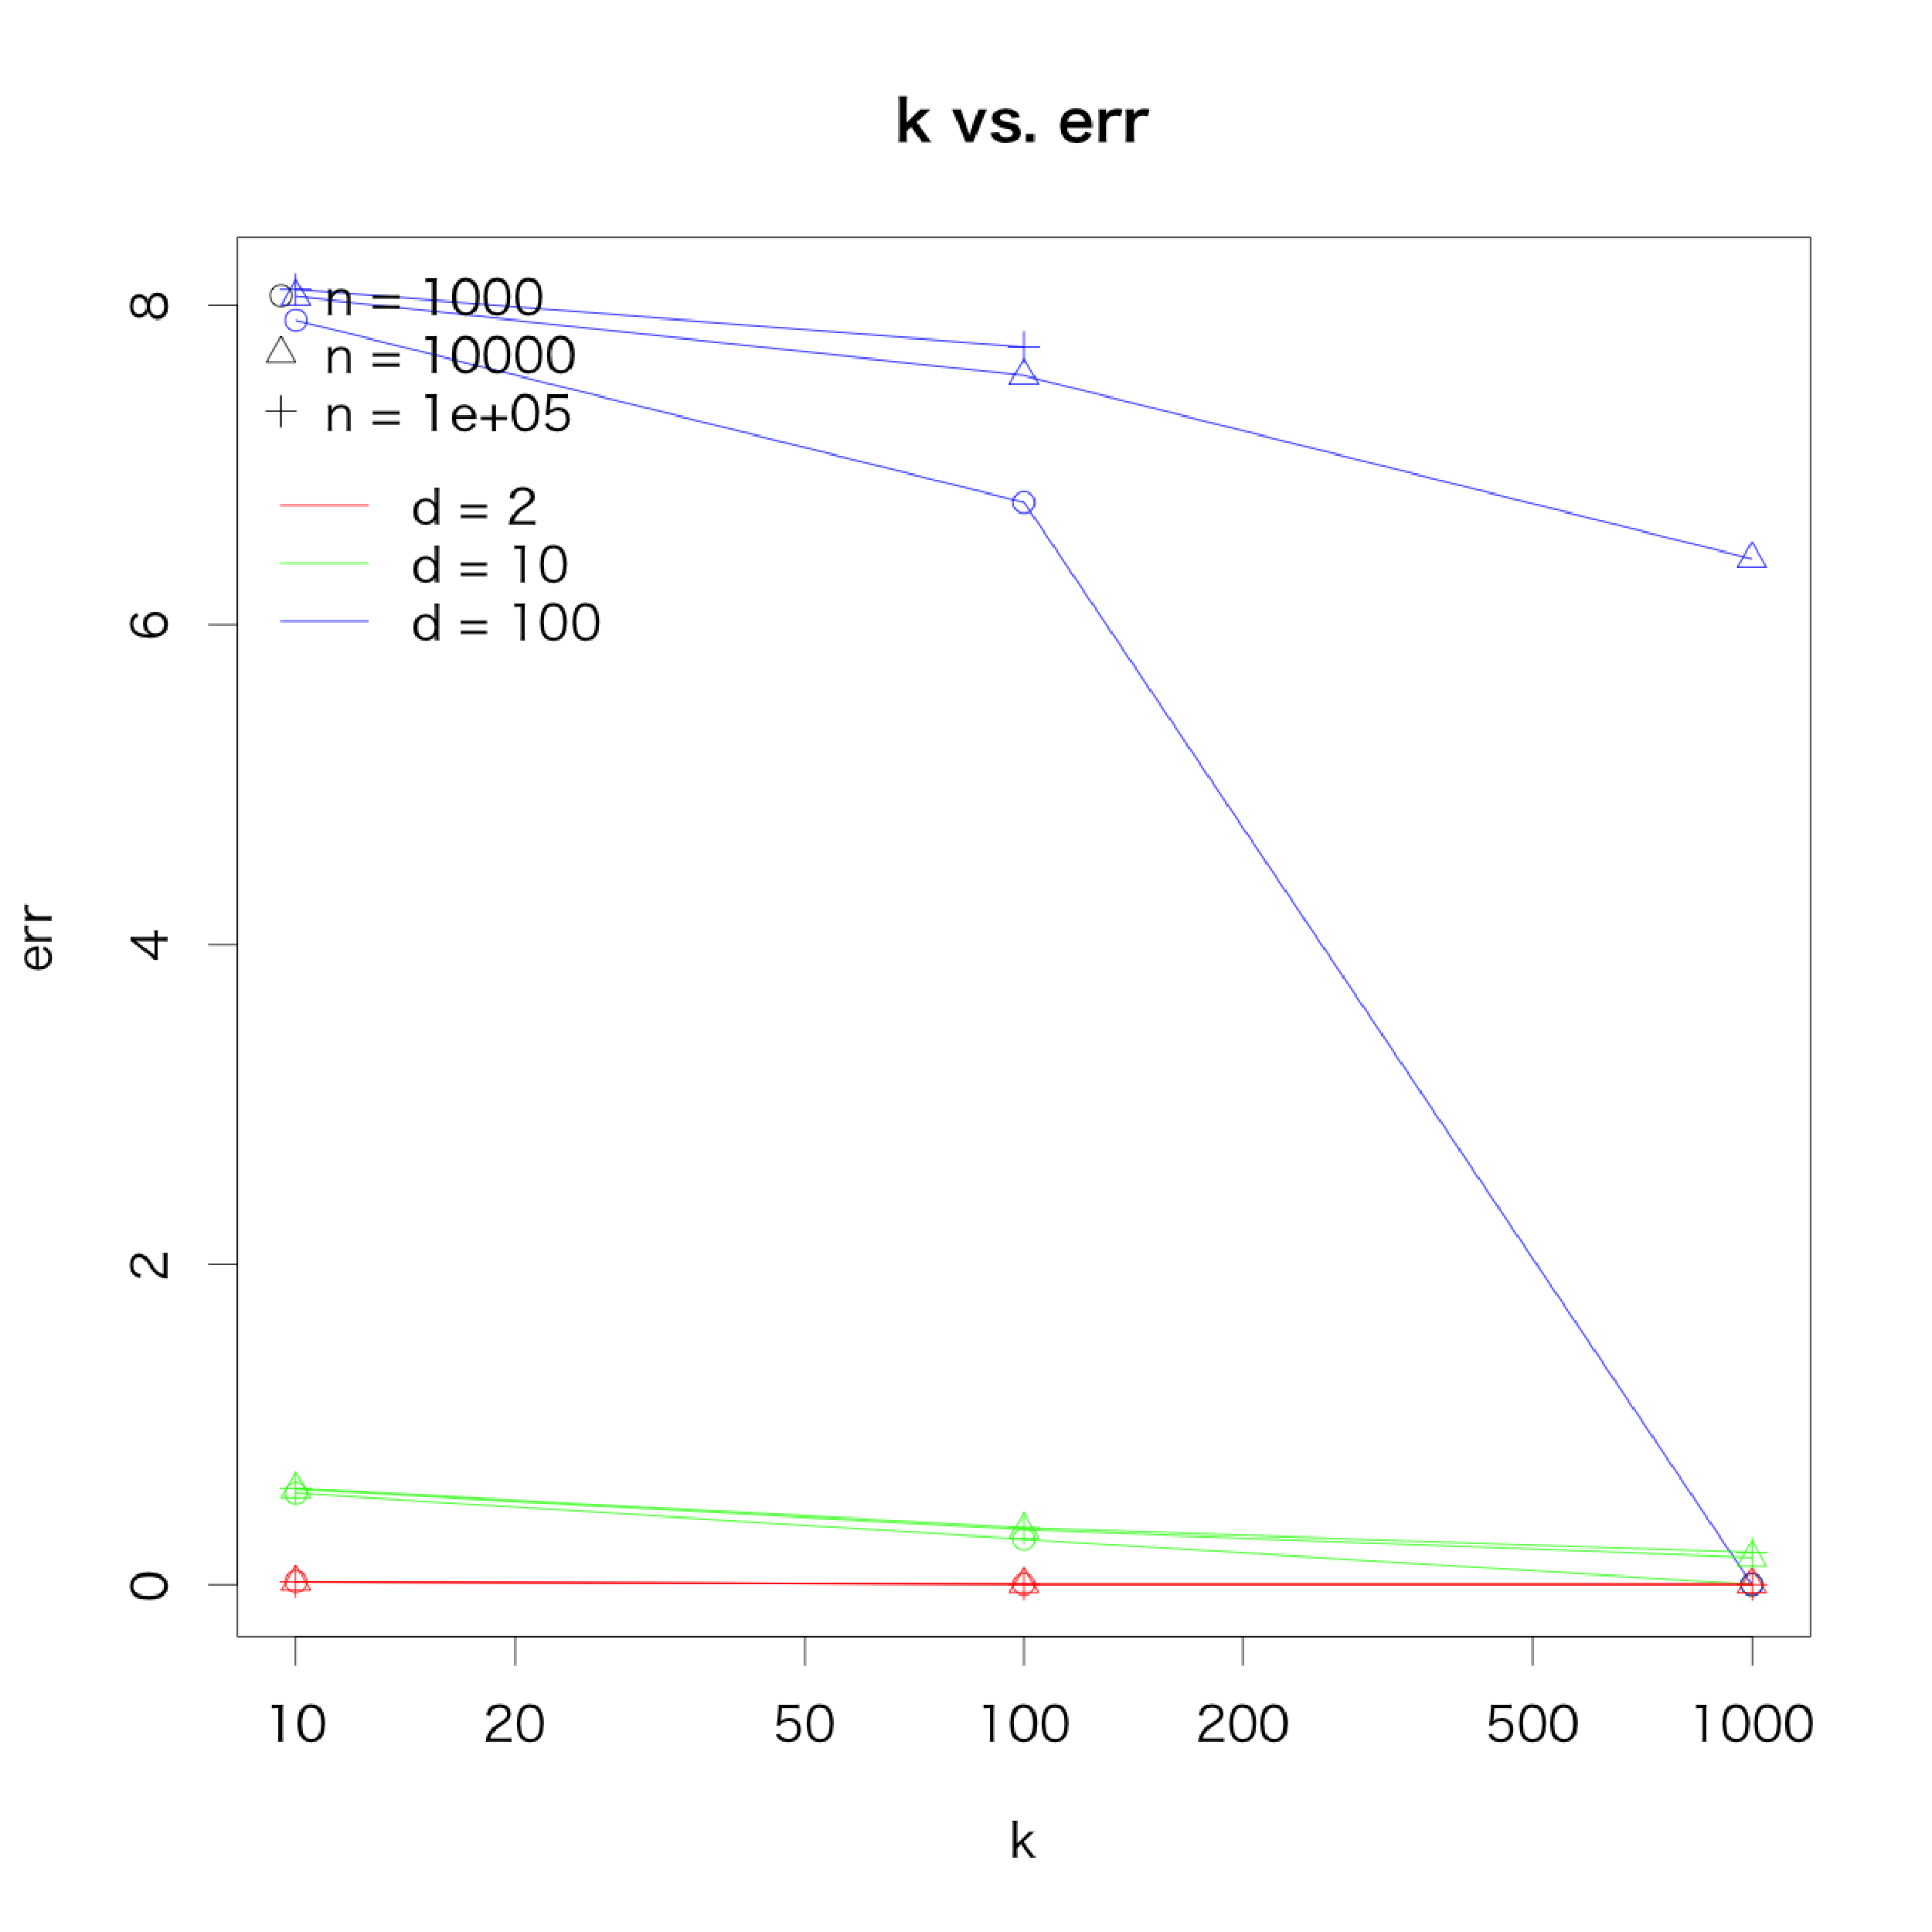
\includegraphics[width=0.33\hsize]{./k_err.pdf}
      &
      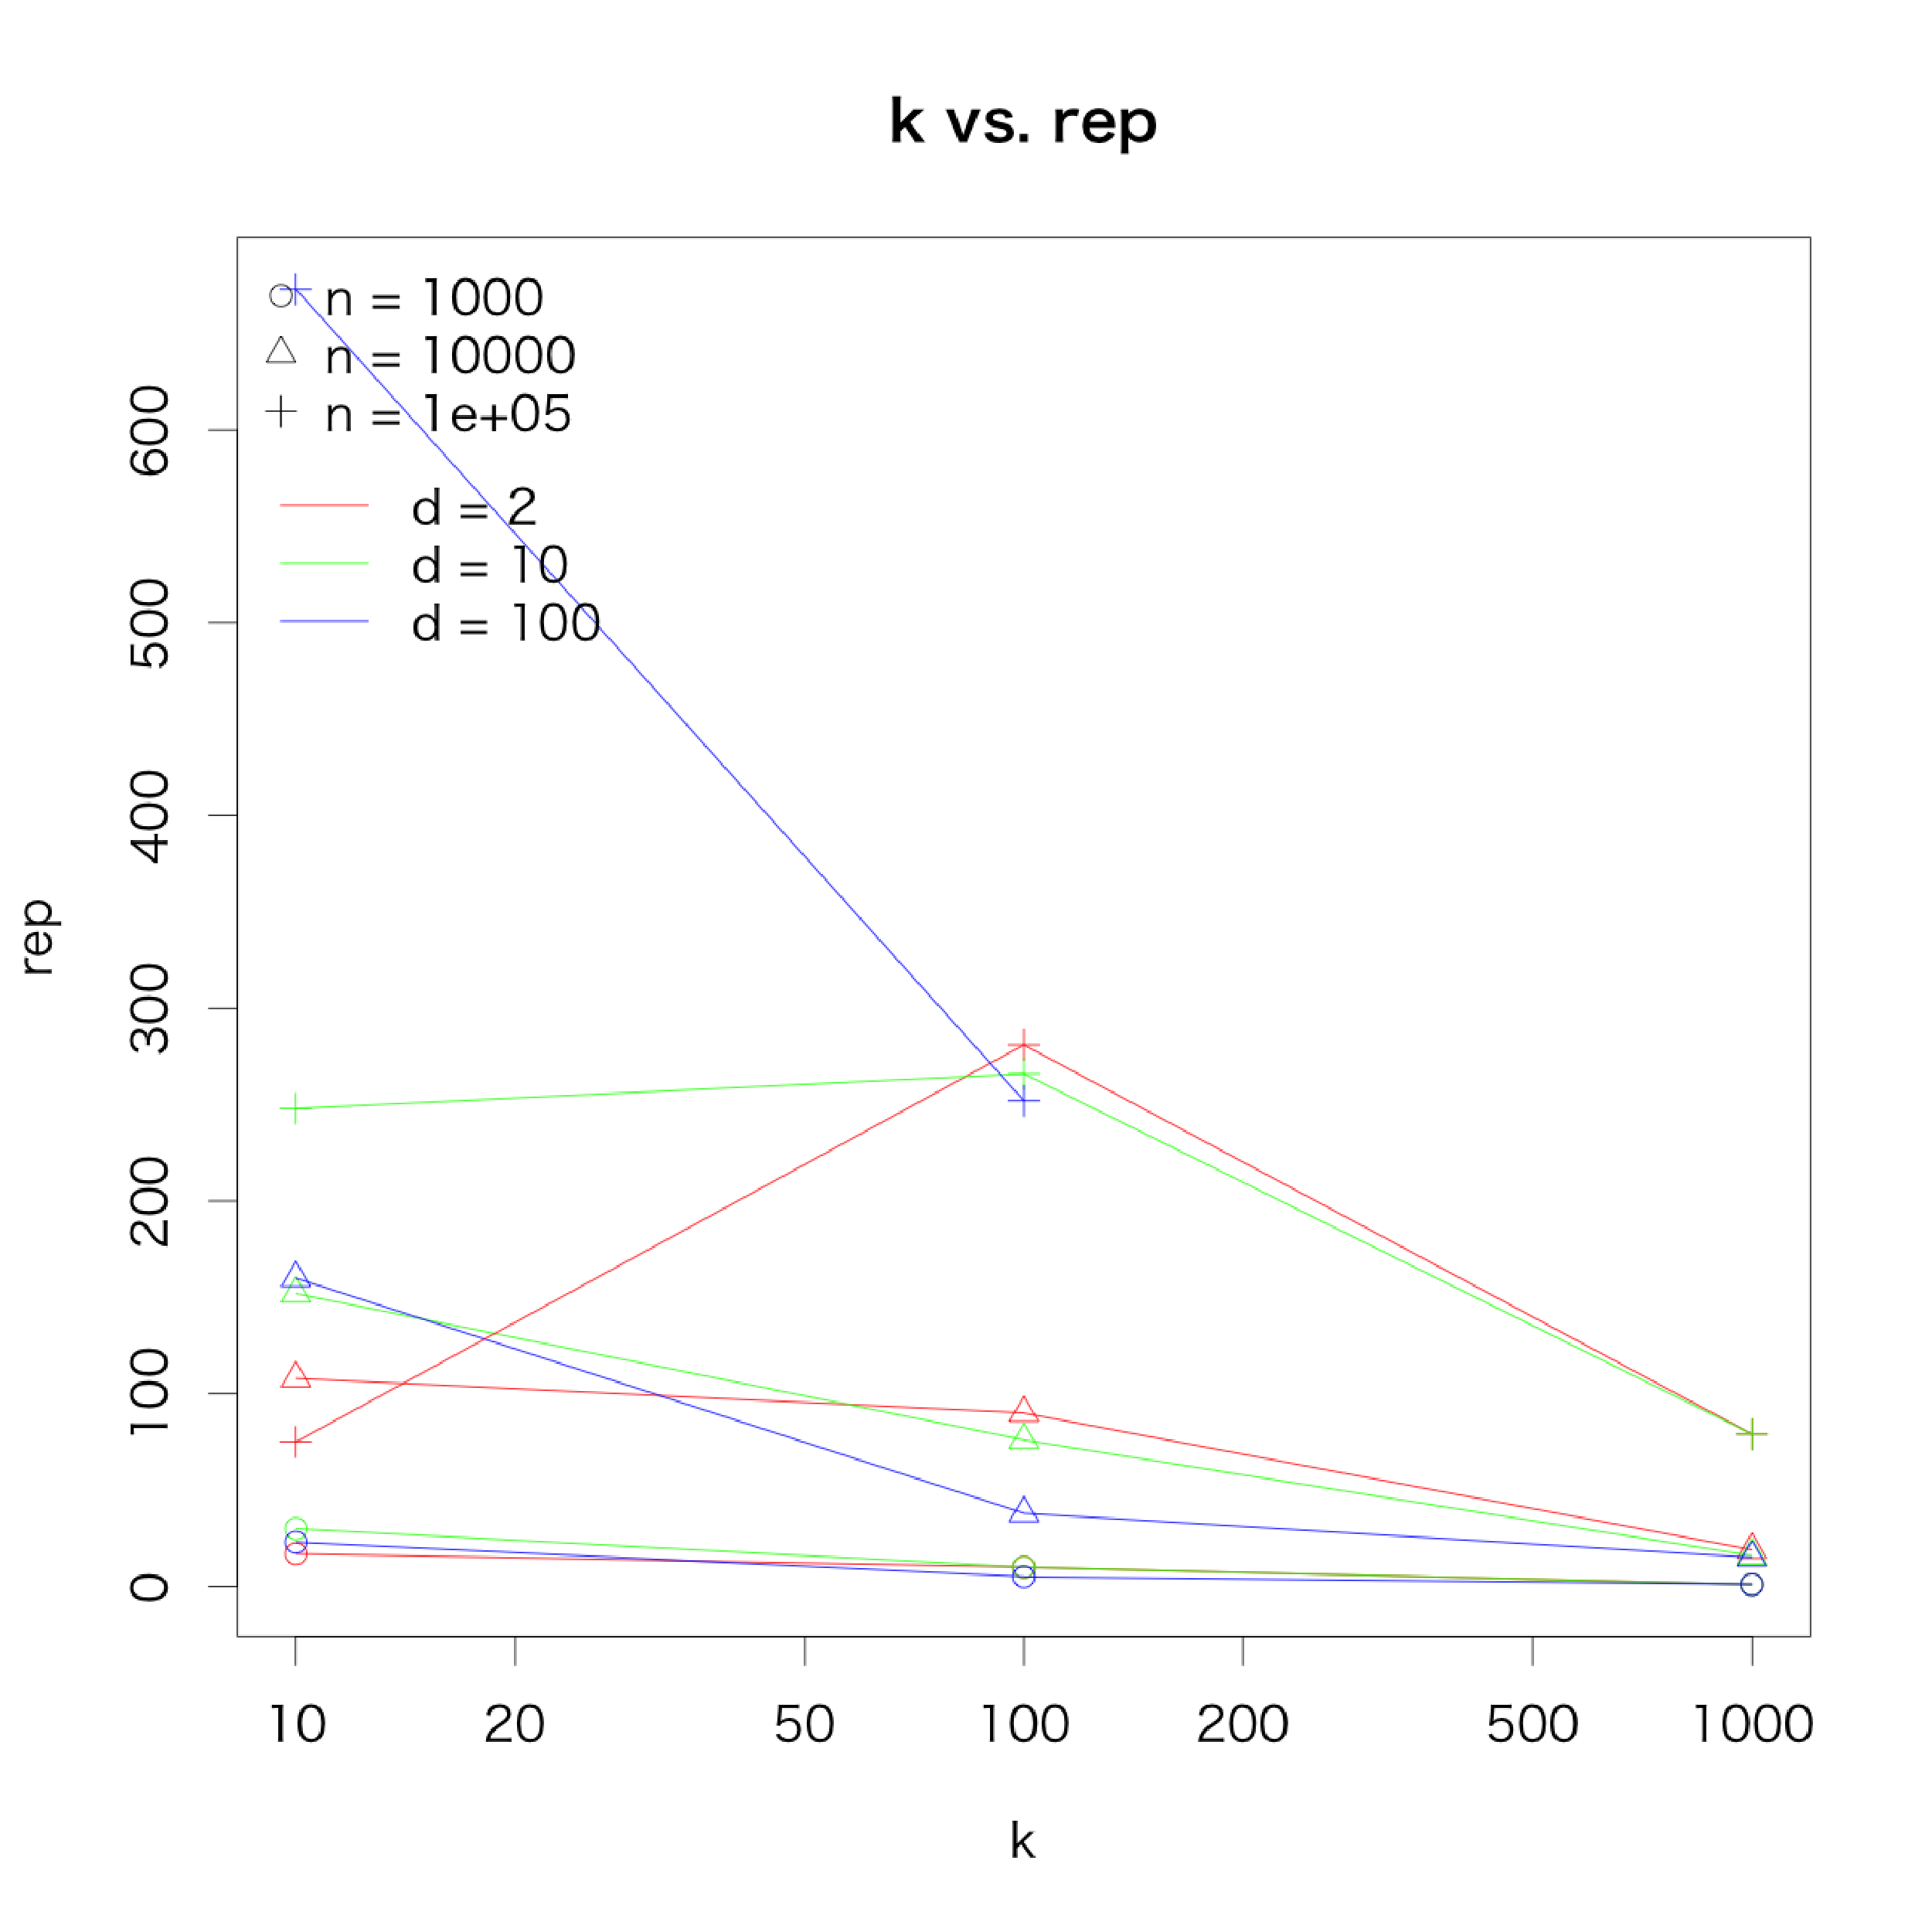
\includegraphics[width=0.33\hsize]{./k_rep.pdf}
  \end{tabular}
  \caption{変数$n$, $d$, $k$を変化させたときのプログラム実行時間(time),平均二乗誤差(err),反復回数(rep)の変化}\label{fig:plot_all}
\end{figure}

図\ref{fig:plot_all}にプロットした結果を示す。プロットはすべて片対数軸で示した。なお,個々のプロットの画像のファイルは,レポートのtexファイルと同じディレクトリ内にある。

\subsection{考察}
\subsubsection{Lloydのk-means法の計算量}
まず,Lloydのk-means法のアルゴリズムの繰り返しステップの計算量について考える。

再クラスタリングの手続きにおいては,各データ点について,最近接のクラスタを探すために$O(k)$の時間がかかり,全データ点について再クラスタリングを行うには$O(nk)$時間かかる。

代表点の再計算については,代表点の重心を考えるためには,各クラスタに属する全ての点の座標を見る必要があるため,全体で$O(n + k)$時間かかる。

これより,繰り返しステップ全体では,$O(nk + n + k) = O(nk)$時間かかると推論できる。

アルゴリズム全体では,この繰り返しステップが何回か繰り返される。何度の繰り返しが必要であるかは,データの性質に依存するため,一般的な解析は難しいが,仮に繰り返し回数を$r$とおくと,全体で$O(rnk)$となると推測できる。

\subsubsection{データ点の数$n$の影響}
まず,データ点数$n$に対して,平均二乗誤差(err)はほぼ一定の値をとった。これは,平均をとる操作をしているため,$n$の大きさに平均二乗誤差は影響を受けないからであると解釈できるだろう。$d = 100$, $k = 1000$の振る舞いが一見不思議に見えるかもしれないが,これは$n = 1000$のとき$k = 1000$と,データ数と等しい数のクラスタに分類すると,誤差が$0$になるということを示しているだけである。

次に,データ点数$n$に対する繰り返し回数(rep)の変化であるが,データによってばらつきがあるものの,$n$の増加に対してほぼ指数の増加をしているとみなしてよいのではなかろうか。

データ点の数$n$に対してプログラムの実行時間はsingle exponentialより早い速度で増加するようだ。これは,先のアルゴリズムの計算量の考察で$O(rnk)$と求めたが,$r$自体が$n$の指数で増加するため,$O(rnk)$全体では$n$の指数よりも速い速度で増加すると推論でき,プログラムの実行結果と符合する。

\subsubsection{次元$d$の影響(「次元の呪い効果の考察」)}
まず,次元の呪いの効果について。次元$d$と平均二乗誤差(err)の関係のグラフを見ると,$d$の増加にしたがって,平均二乗誤差は急速に増加していることがわかる。増加の速度は一重指数よりも速く,$(k = 1000, n = 1000)$を除く全てのサンプルで同様の結果が得られれている。これは,高次元になると,点同士の間隔が互いに粗になり,クラスタ内での分散が大きくなってしまうというふうに解釈できる。まさに「次元の呪い」効果の一例であろう。$(k = 1000, n = 1000)$のサンプルにて次元の呪い効果が見られなかった理由は,各点を個々のクラスタとみなした場合に平均二乗誤差が0となるからである。

次に,次元の大きさと繰り返し回数(rep)について。これは,$(k = 10, n = 100000)$のサンプルを除いてほぼ一定とみてよいだろう。$(k = 10, n = 100000)$のケースだけ例外的であった理由は,次の通りである。このパラメタの組合せの場合,解としてありえるクラスタリングの数が他のパラメタよりも多くなる。このため,膨大な解空間の中で,現在の解の近傍を渡り歩きながら最適解を探索するために必要な繰り返し回数が多くなったと解釈できるだろう。

最後に次元の大きさとプログラムの実行時間について。次元の大きさによらずほぼ一定の結果と考えることができるが,$n$が大きい場合には,プログラムの実行時間が長くなるという傾向が見られた。これについては,先に$n$の効果のところで見たとおりである。

\subsubsection{クラスタ数$k$の影響}
クラスタ数$k$を増やすことにより,平均二乗誤差は小さくなる。また,クラスタ数を大きくしたほうが,繰り返し回数が小さくなる傾向にあるのは,解空間が小さくなることによるものであろう。最後に,クラスタ数とプログラムの実行時間であるが,$k$の増加にたいして指数的に実行時間が増加している。繰り返し回数$r$の減少も加味して,プログラム実行時間の$k$に対する指数増加の説明を考えようとしたが,これについてはあまり良くわからなかった。

\section{高速化の実装}
\section{生物データでの比較}
これらについては,まだ試していません。

%%%%%%%%%%%%%%%%%%%%%%%%%%%%%%%%%%%%%%%%%%%%%%%%%%%%%%%%%
\end{document}

